\documentclass{article}
\usepackage[utf8]{inputenc}
\usepackage{hyperref}
\usepackage{graphicx}
\usepackage{float}


\hypersetup{
    colorlinks,
    citecolor=blue,
    filecolor=blue,
    linkcolor=blue,
    urlcolor=blue
}

\title{Progetto di Ingegneria del Software: Team3}
\author{Juan Guillermo Jaramillo Saa (SM)\\
  \texttt{juan.jaramillosaa@studio.unibo.it}
  \and
  Daniele Tarek Iaisy (PO)\\
  \texttt{danieletarek.iaisy@studio.unibo.it}
  \and
  Alexandru Bogdan Nicolescu (DEV)\\
  \texttt{alexandru.nicolescu@studio.unibo.it}
  \and
  Riccardo Fava (DEV)\\
  \texttt{riccardo.fava5@studio.unibo.it}
  \and
  Andrea Largura (DEV)\\
  \texttt{andrea.largura@studio.unibo.it}}
\date{14 Dicembre 2022}

\begin{document}
\maketitle
\pagebreak
\tableofcontents
\pagebreak
\section{Prodotto}
\subsection{Descrizione del prodotto}
Si vuole costruire un prodotto software capace di raccolta e analisi dei tweet di Twitter. \\ 
I tweet possono riferirsi ad una persona, ad un luogo, ad un evento, ad un gioco, ad una trasmissione televisiva. \\
Si vogliono utilizzare i tweet anche per giocare in gruppo o supportare giochi televisivi. \\
Le sezioni a seguire riportano le funzionalit\'a che si vogliono implementare.
\subsection{Ricerca}
\begin{itemize}
    \item Per parola chiave: vengono restituiti i tweet contenenti una data parola chiave
    \item Username: vengono restituiti i tweet pubblicati da un dato utente
    \item Hashtag: vengono restituiti i tweet per un dato hashtag
\end{itemize}
È inoltre possibile scegliere se attivare lo streaming dei tweet in tempo reale.
\subsubsection{Filtraggio}
\begin{itemize}
    \item Per data: è possibile scegliere gli estremi dell’arco temporale preferito (all’interno dell’ultima settimana)
    \item Per numero di risultati: è possibile scegliere il numero di risultati da visualizzare
\end{itemize}

\subsubsection{Statistiche}
\begin{itemize}
    \item Sentiment analysis: ogni tweet riceve un punteggio (Buono, Neutro, Male).
    \item Sentiment analysis della ricerca: ogni ricerca genera un diagramma con parole positive, negative e neutre utilizzate nell'intera ricerca.
    \item Wordcloud: diagramma delle parole più ricorrenti all’interno della ricerca.
\end{itemize}
\subsection{Epiche}
\begin{itemize}
    \item L'eredit\'a: deve essere possibile raccogliere i tweet di chi prova a indovinare la ghigliottina, per visualizzare (in ordine temporale, o su una mappa) tutti coloro che indovinano
    \item Scacchi: deve essere possibile poter giocare a scacchi in modo tale che le mosse avversarie siano scelte per maggioranza
    \item Fantacitorio: deve essere possibile raccogliere i tweet delle squadre del fantacitorio o di un utente in particolare e anche visualizzare una classifica con politici e punti (e il miglior punteggio singolare di tutta la classifica).
\end{itemize}
\subsection{Backlog di prodotto}
\begin{itemize}
    \item \textbf{US}: Homepage \\
    \textbf{Descrizione}: Come visitatore di pagine web vorrei poter visualizzare la homepage dell'applicazione \\
    \textbf{Punti}: 8
    \item \textbf{US}: Ricerca per parola chiave \\
    \textbf{Descrizione}: Come abitante di una bolla, voglio filtrare i tweet per parola chiave, così da vedere solo quello che interessa a me \\
    \textbf{Punti}: 13
    \item \textbf{US}: Ricerca per utente \\
    \textbf{Descrizione}: Come genitore apprensivo vorrei un modo per cercare i tweet di mio figlio per monitorarlo \\
    \textbf{Punti}: 15
    \item \textbf{US}: Visualizzazione diagramma a barre \\
    \textbf{Descrizione}: Come analista vorrei avere un grafico che mi permette di vedere il numero di tweet raccolti nel tempo, così da sapere gli andamenti di popolarità dei topic \\
    \textbf{Punti}: 13
    \item \textbf{US}: Visualizzazione tweet su mappa \\
    \textbf{Descrizione}: Come genitore apprensivo vorrei un modo per cercare i tweet di mio figlio e visualizzarli sulla mappa \\
    \textbf{Punti}: 13
    \item \textbf{US}: Visualizzazione sentiment analysis \\
    \textbf{Descrizione}: Come analista di dati vorrei un grafico a torta sul sentiment dei tweet, per farmi un'idea di cosa ne pensino gli utenti \\
    \textbf{Punti}: 28
    \item \textbf{US}: Ricerca per data \\
    \textbf{Descrizione}: Come storico, voglio poter scegliere un intervallo di date, per selezionare i tweet del solo periodo che sto studiando \\
    \textbf{Punti}: 14
    \item \textbf{US}: Scelta del numero dei risultati \\
    \textbf{Descrizione}: Come binge tweeter, voglio poter visualizzare piu' di 10 tweet alla volta \\
    \textbf{Punti}: 15
    \item \textbf{US}: Visualizzazione term cloud \\
    \textbf{Descrizione}: Come membro dell'accademia della crusca vorrei vedere le parole dei tweet selezionati su una term cloud, così da poter vedere le parole più utilizzate \\
    \textbf{Punti}: 13
    \item \textbf{US}: La ghigliottina \\
    \textbf{Descrizione}: Come spettatore de \#leredita (RAI1) voglio raccogliere i tweet di chi prova a indovinare la ghigliottina, per visualizzare (in ordine temporale, o su una mappa) tutti coloro che indovinano \\
    \textbf{Punti}: 32
    \item \textbf{US}: Proposta sfida \\
    \textbf{Descrizione}: Come giocatore di scacchi voglio sfidare gruppi di persone in rete, per giocare partite le cui mosse verranno scelte a maggioranza \\
    \textbf{Punti}: 18
    \item \textbf{US}: Mossa sfida \\
    \textbf{Descrizione}: Come giocatore di scacchi, voglio raccogliere i tweet che rispondono alla mia mossa, per scegliere e visualizzare la mossa scelta dalla maggioranza \\
    \textbf{Punti}: 23
    \item \textbf{US}: Punteggi settimanali \\
    \textbf{Descrizione}: Come spettatore del fantacitorio voglio poter visualizzare la classifica emendabile settimanale \/ di sempre dei politici. \\
    \textbf{Punti}: 26
    \item \textbf{US}: Immagini squadre \\
    \textbf{Descrizione}: Come spettatore del fantacitorio voglio poter sfogliare le immagini delle squadre registrate \\
    \textbf{Punti}: 24
    \item \textbf{US}: Squadra utente \\
    \textbf{Descrizione}: Come spettatore del fantacitorio voglio poter vedere le squadre dei miei amici \\
    \textbf{Punti}: 19
\end{itemize}
\section{ Diagrammi }
Questi diagrammi sono stati fatti tramite lo strumento open source plantuml \href{https://plantuml.com/}{https://plantuml.com/}. 

Si tratta di uno strumento che permette di creare diagrammi a partire da testo.
\subsection{Caso d'uso iniziale}
\begin{figure}[H]
    \centering
    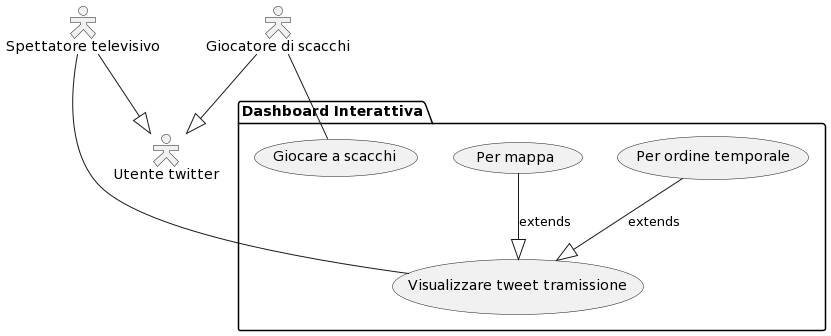
\includegraphics[scale=0.40]{diagrammi/usecaseEpiche.png}
    \caption{Caso d'uso, parte 1}
    \label{fig:usecase1}
\end{figure}
\begin{figure}[H]
    \centering
    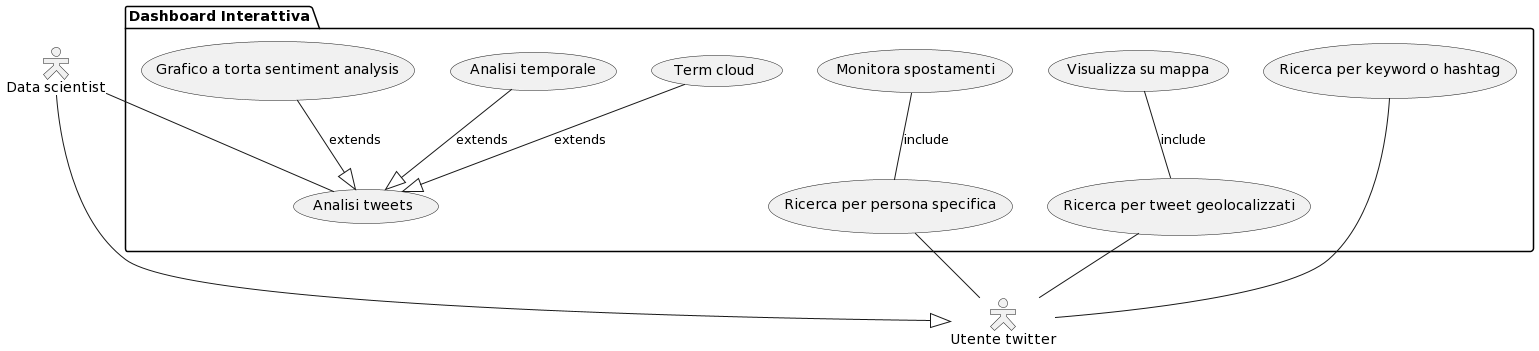
\includegraphics[scale=0.30]{diagrammi/usecaseScenario.png}
    \caption{Caso d'uso, parte 2}
    \label{fig:usecase2}
\end{figure}
\subsection{Caso d'uso (aggiunto)}
\begin{figure}[H]
    \centering
    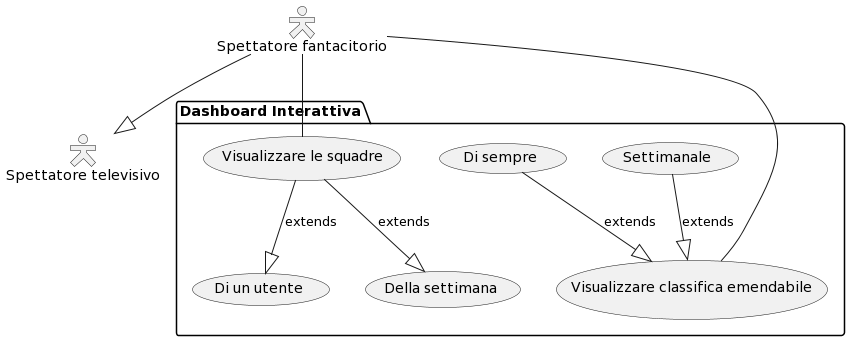
\includegraphics[scale=0.40]{diagrammi/usecaseAggiunta.png}
    \caption{Caso d'uso, parte 3 (aggiunta dello sprint 4)}
    \label{fig:usecase2}
\end{figure}
\subsection{Diagramma di Deployment}
\begin{figure}[H]
    \centering
    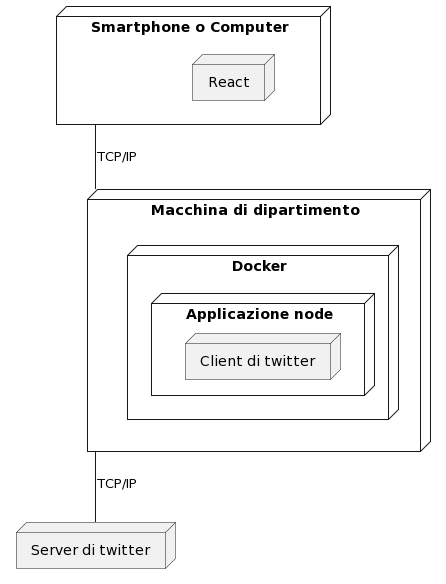
\includegraphics[scale=0.33]{diagrammi/deployment.png}
    \caption{Diagramma di deployment}
    \label{fig:deployment}
\end{figure}
\subsection{Continuous Integration, Continuous Deployment}
Quando viene effettuato un push sul main viene effettuata l'integrazione con l'aggiornamento degli item su \textit{Taiga} (se vengono trovati messaggi con TG-\#task \#staus). \\
Dopodich\'e vengono fatti partire gli stage di test, build e deploy automatizzato. \\
In questo modo abbiamo \href{http://site212236.tw.cs.unibo.it/}{http://site212236.tw.cs.unibo.it} sempre aggiornato all'ultima versione. \\
Visto che abbiamo adottato \href{https://docs.github.com/en/get-started/quickstart/github-flow}{GitHub Workflow} come flusso di lavoro git, ci \`e stato utile attivare degli stage ad-hoc per le merge request. \\
Quando viene effettuata una merge request, viene fatto partire lo stage di test e di build, in questo modo riuscivamo a capire fin da subito se i nostri branch fossero parzialmente pronti ad essere mergiati al main (non prima di essere stati visionati da almeno un altro sviluppatore)
\begin{figure}[H]
    \centering
    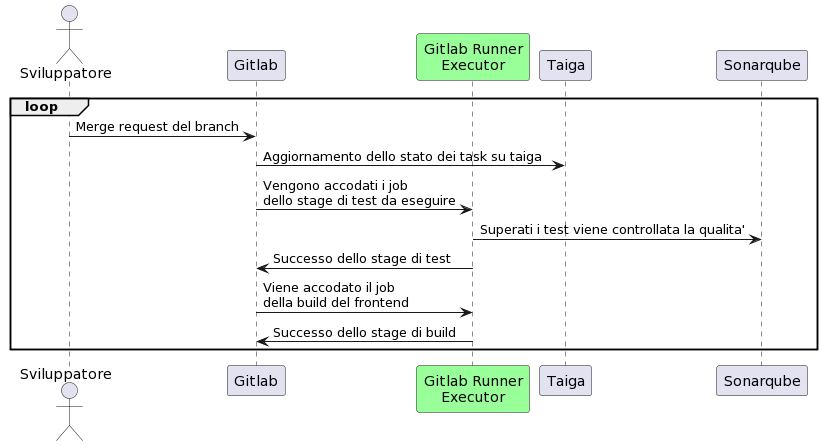
\includegraphics[scale=0.38]{diagrammi/mergecicd.png}
    \caption{Diagramma di sequenza, merge requests}
    \label{fig:deployment}
\end{figure}
\begin{figure}[H]
    \centering
    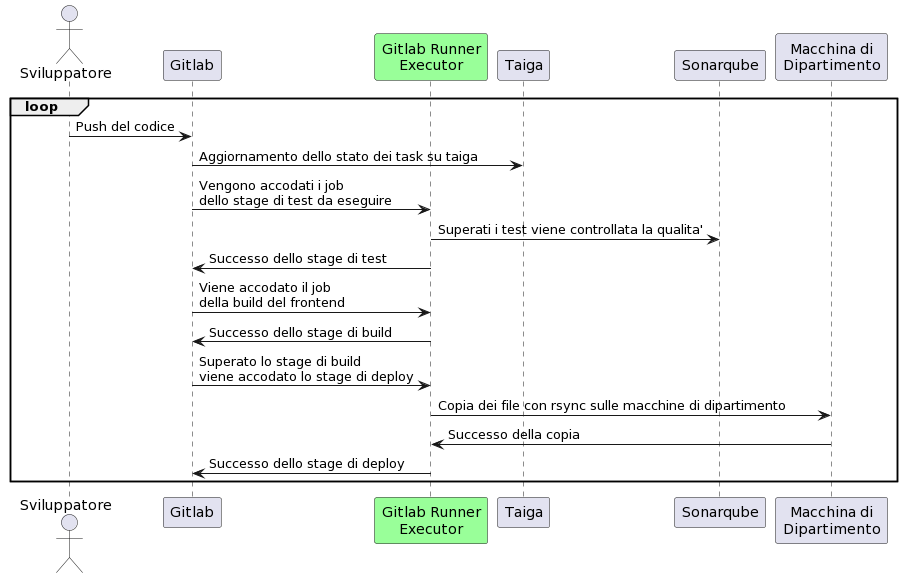
\includegraphics[scale=0.38]{diagrammi/cicd.png}
    \caption{Diagramma di sequenza, main}
    \label{fig:deployment}
\end{figure}
\section{Sprint}
\subsection{Sprint 0}
\subsubsection{ Team building }
Il team \`e stato creato grazie a Trello, prima di questo progetto solo Juan e Alex si conoscevano.

Per questo motivo abbiamo speso la maggior parte di questo sprint a conoscerci tra di noi.

\subsubsection{ Scrumble }
Abbiamo effettuato la partita di scrumble in modalit\'a mista (tramite \textit{Discord}), con Daniele che ha condiviso lo schermo.

\begin{figure}[H]
    \centering
    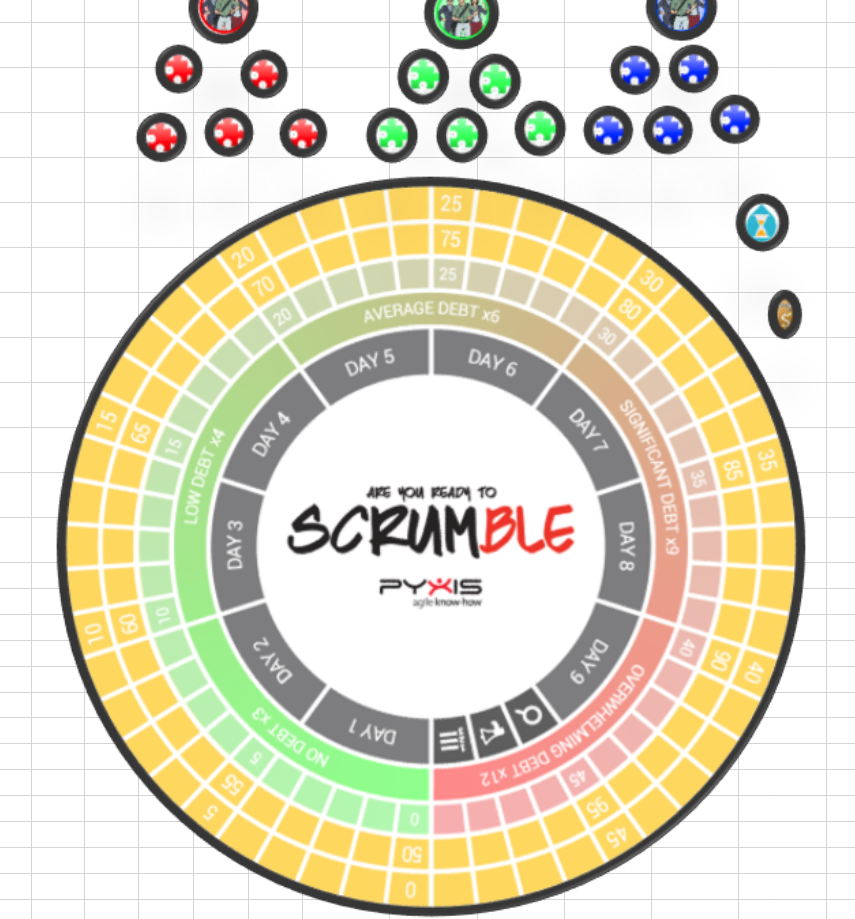
\includegraphics[scale=0.30]{scrumble/scrumble_board.png}
    \caption{Screenshot della board che abbiamo utilizzato}
    \label{fig:scrumbleboard}
\end{figure}

La partita, in linea generale, \`e andata bene, siamo riusciti a rompere il ghiaccio per conoscerci meglio e i ruoli intrapresi durante la partita sono rimasti tali per l'intero progetto.
\subsubsection{ Scheda di autovalutazione }
Al termine della partita abbiamo provveduto a compilare la scheda di autovalutazione, riportata a seguire:

\begin{figure}[H]
    \centering
    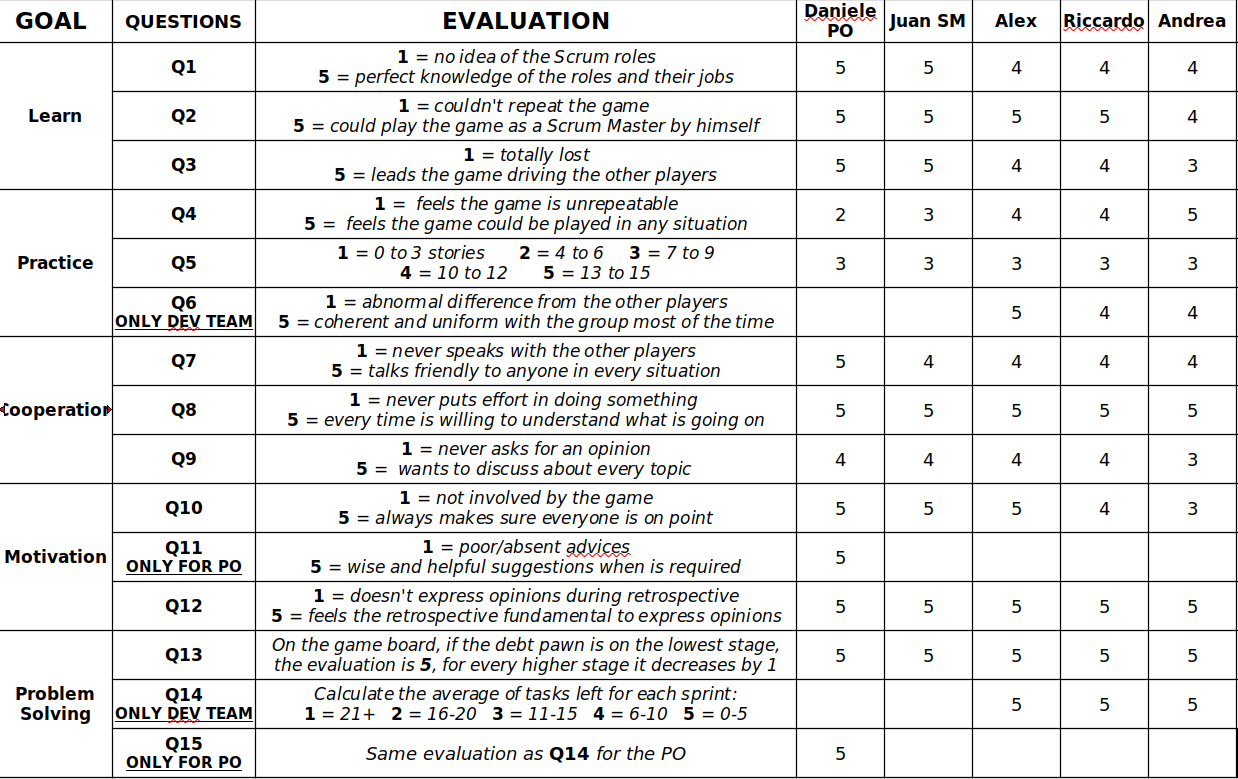
\includegraphics[scale=0.30]{scrumble/autovalutazione.png}
    \caption{Screenshot della scheda da LibreOffice}
    \label{fig:scrumbleautovalutazione}
\end{figure}

\subsubsection{Flusso di lavoro}
Abbiamo deciso di utilizzare il \href{https://docs.github.com/en/get-started/quickstart/github-flow}{GitHub Workflow}.

Nel nostro caso, abbiamo deciso che ai task delle US, se possibile, avremmo associato feature branch su cui sviluppare e completare i singoli task, per poi effettuare una merge request al branch main che sarebbe stata approvata in seguito.
\begin{figure}[H]
    \centering
    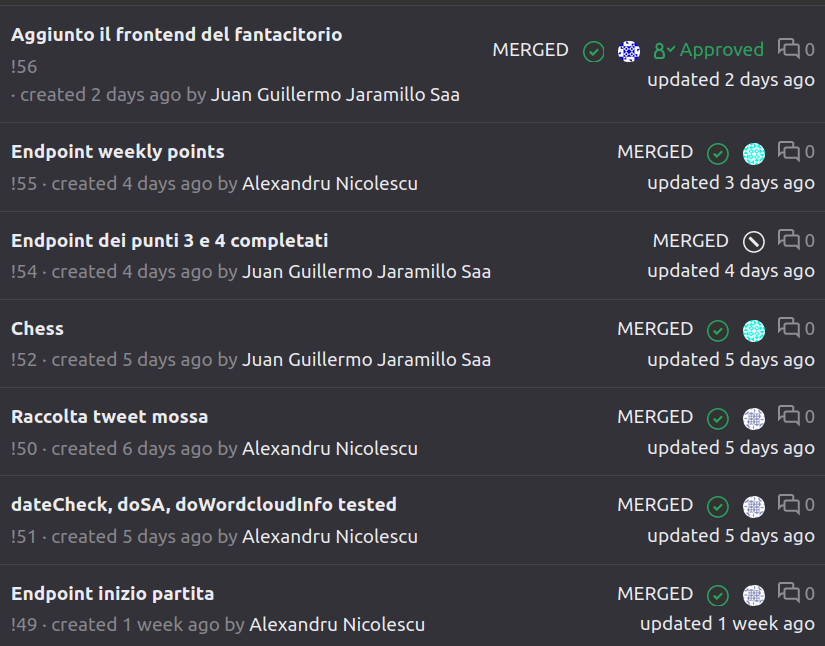
\includegraphics[scale=0.23]{misc/mergerequests.png}
    \caption{Screenshot da Gitlab}
    \label{fig:mergerequests}
\end{figure}
\subsection{Sprint 1}
\subsubsection{Sprint goal}
Il nostro obiettivo fin da questo sprint \`e stato quello di portare un client che potesse effettuare ricerche di tweet per parola chiave. \\
Ci \`e sembrato un buon obiettivo da raggiungere nelle prime due settimane di lavoro.
\subsubsection{Sprint backlog}
\begin{itemize}
    \item Come abitante di una bolla, voglio filtrare i tweet per parola chiave, così da vedere solo quello che interessa a me

    \textbf{Stima}: 8 punti
    \item Come visitatore di pagine web vorrei poter visualizzare la homepage dell'applicazione

    \textbf{Stima}: 13 punti
\end{itemize}
\subsubsection{Definition of Done}
Questo \`e stato uno dei punti dolenti di questo sprint: essendoci concentrati molto sul portare delle funzionalit\'a al prof, abbiamo trascurato la DOD. 

In generale, durante questo sprint abbiamo considerato una US \textit{closed} quando era implementato ci\'o che ne era richiesto dalla US su taiga.
\subsubsection{Burndown dello sprint}
\begin{figure}[H]
    \centering
    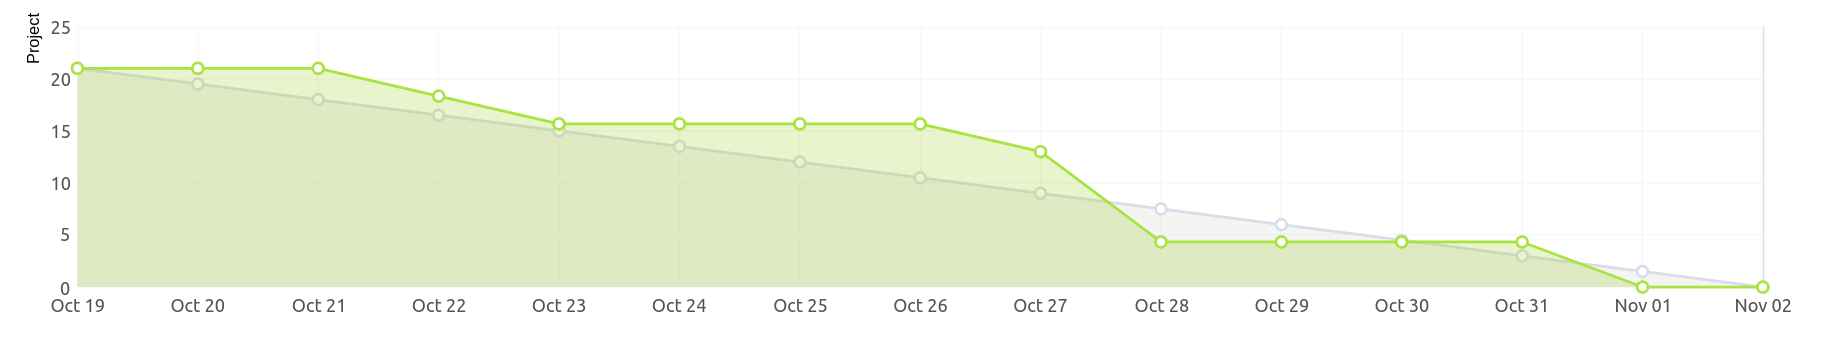
\includegraphics[scale=0.22]{burdowns/sprint1.png}
    \caption{Screenshot da Taiga}
    \label{fig:burndown1}
\end{figure}
\subsubsection{Test}
Purtroppo in questo sprint non siamo riusciti a scrivere nemmeno un test, abbiamo cercato di recuperare a partire dallo sprint 2.
\subsubsection{Scelte progettuali}
Questo \`e stato uno sprint importante anche per la scelta delle tecnologie da utilizzare per realizzare il prodotto. 

Poich\`e alcuni di noi erano gi\'a familiari allo sviluppo di applicazioni web con React e Node, abbiamo deciso di realizzare una web application con le seguenti tecnologie:
\begin{itemize}
    \item React per il frontend (con l'utilizzo di una libreria per la gestione dello stato, \href{https://redux.js.org/}{Redux})
    \item \href{https://tailwindcss.com/}{Tailwind CSS} come framework css
    \item Node per il backend (per interfacciarsi con le API di twitter)
\end{itemize}
Per fare in modo che tutti si trovassero allo stesso livello con le tecnologie scelte e con gli strumenti CAS, abbiamo creato degli \textit{Storyless tasks} su Taiga, quali:
\begin{itemize}
    \item Studio di react + redux
    \item Studio delle API di twitter (v2)
    \item Studio di Taiga
\end{itemize}
\subsubsection{Sprint Review}
Grazie alla Sprint Review siamo riusciti a capire che la nostra US riguardante la Homepage del sito fosse ridondante e non richiesta.

Ne abbiamo preso atto per gli sprint successivi.
\subsubsection{Retrospettiva}
In questo sprint abbiamo cominciato a capire la vera natura di Scrum oltre a conoscerci meglio tra di noi perche' se non per Juan e Alex che si conoscevano da prima, tutti gli altri membri del team non si conoscevano tra loro.

Proprio perche' non avevamo mai lavorato con Scrum, abbiamo commesso degli errori abbastanza gravi:
\begin{itemize}
    \item Durante lo sprint planning abbiamo trascurato la DOD.
    \item Stessa cosa \`e successa con lo sprint goal.
    \item Poich\`e ci siamo concentrati tantissimo sullo scrivere codice, abbiamo trascurato del tutto la parte di testing, non abbiamo scritto alcun test.
\end{itemize}
\begin{figure}[H]
    \centering
    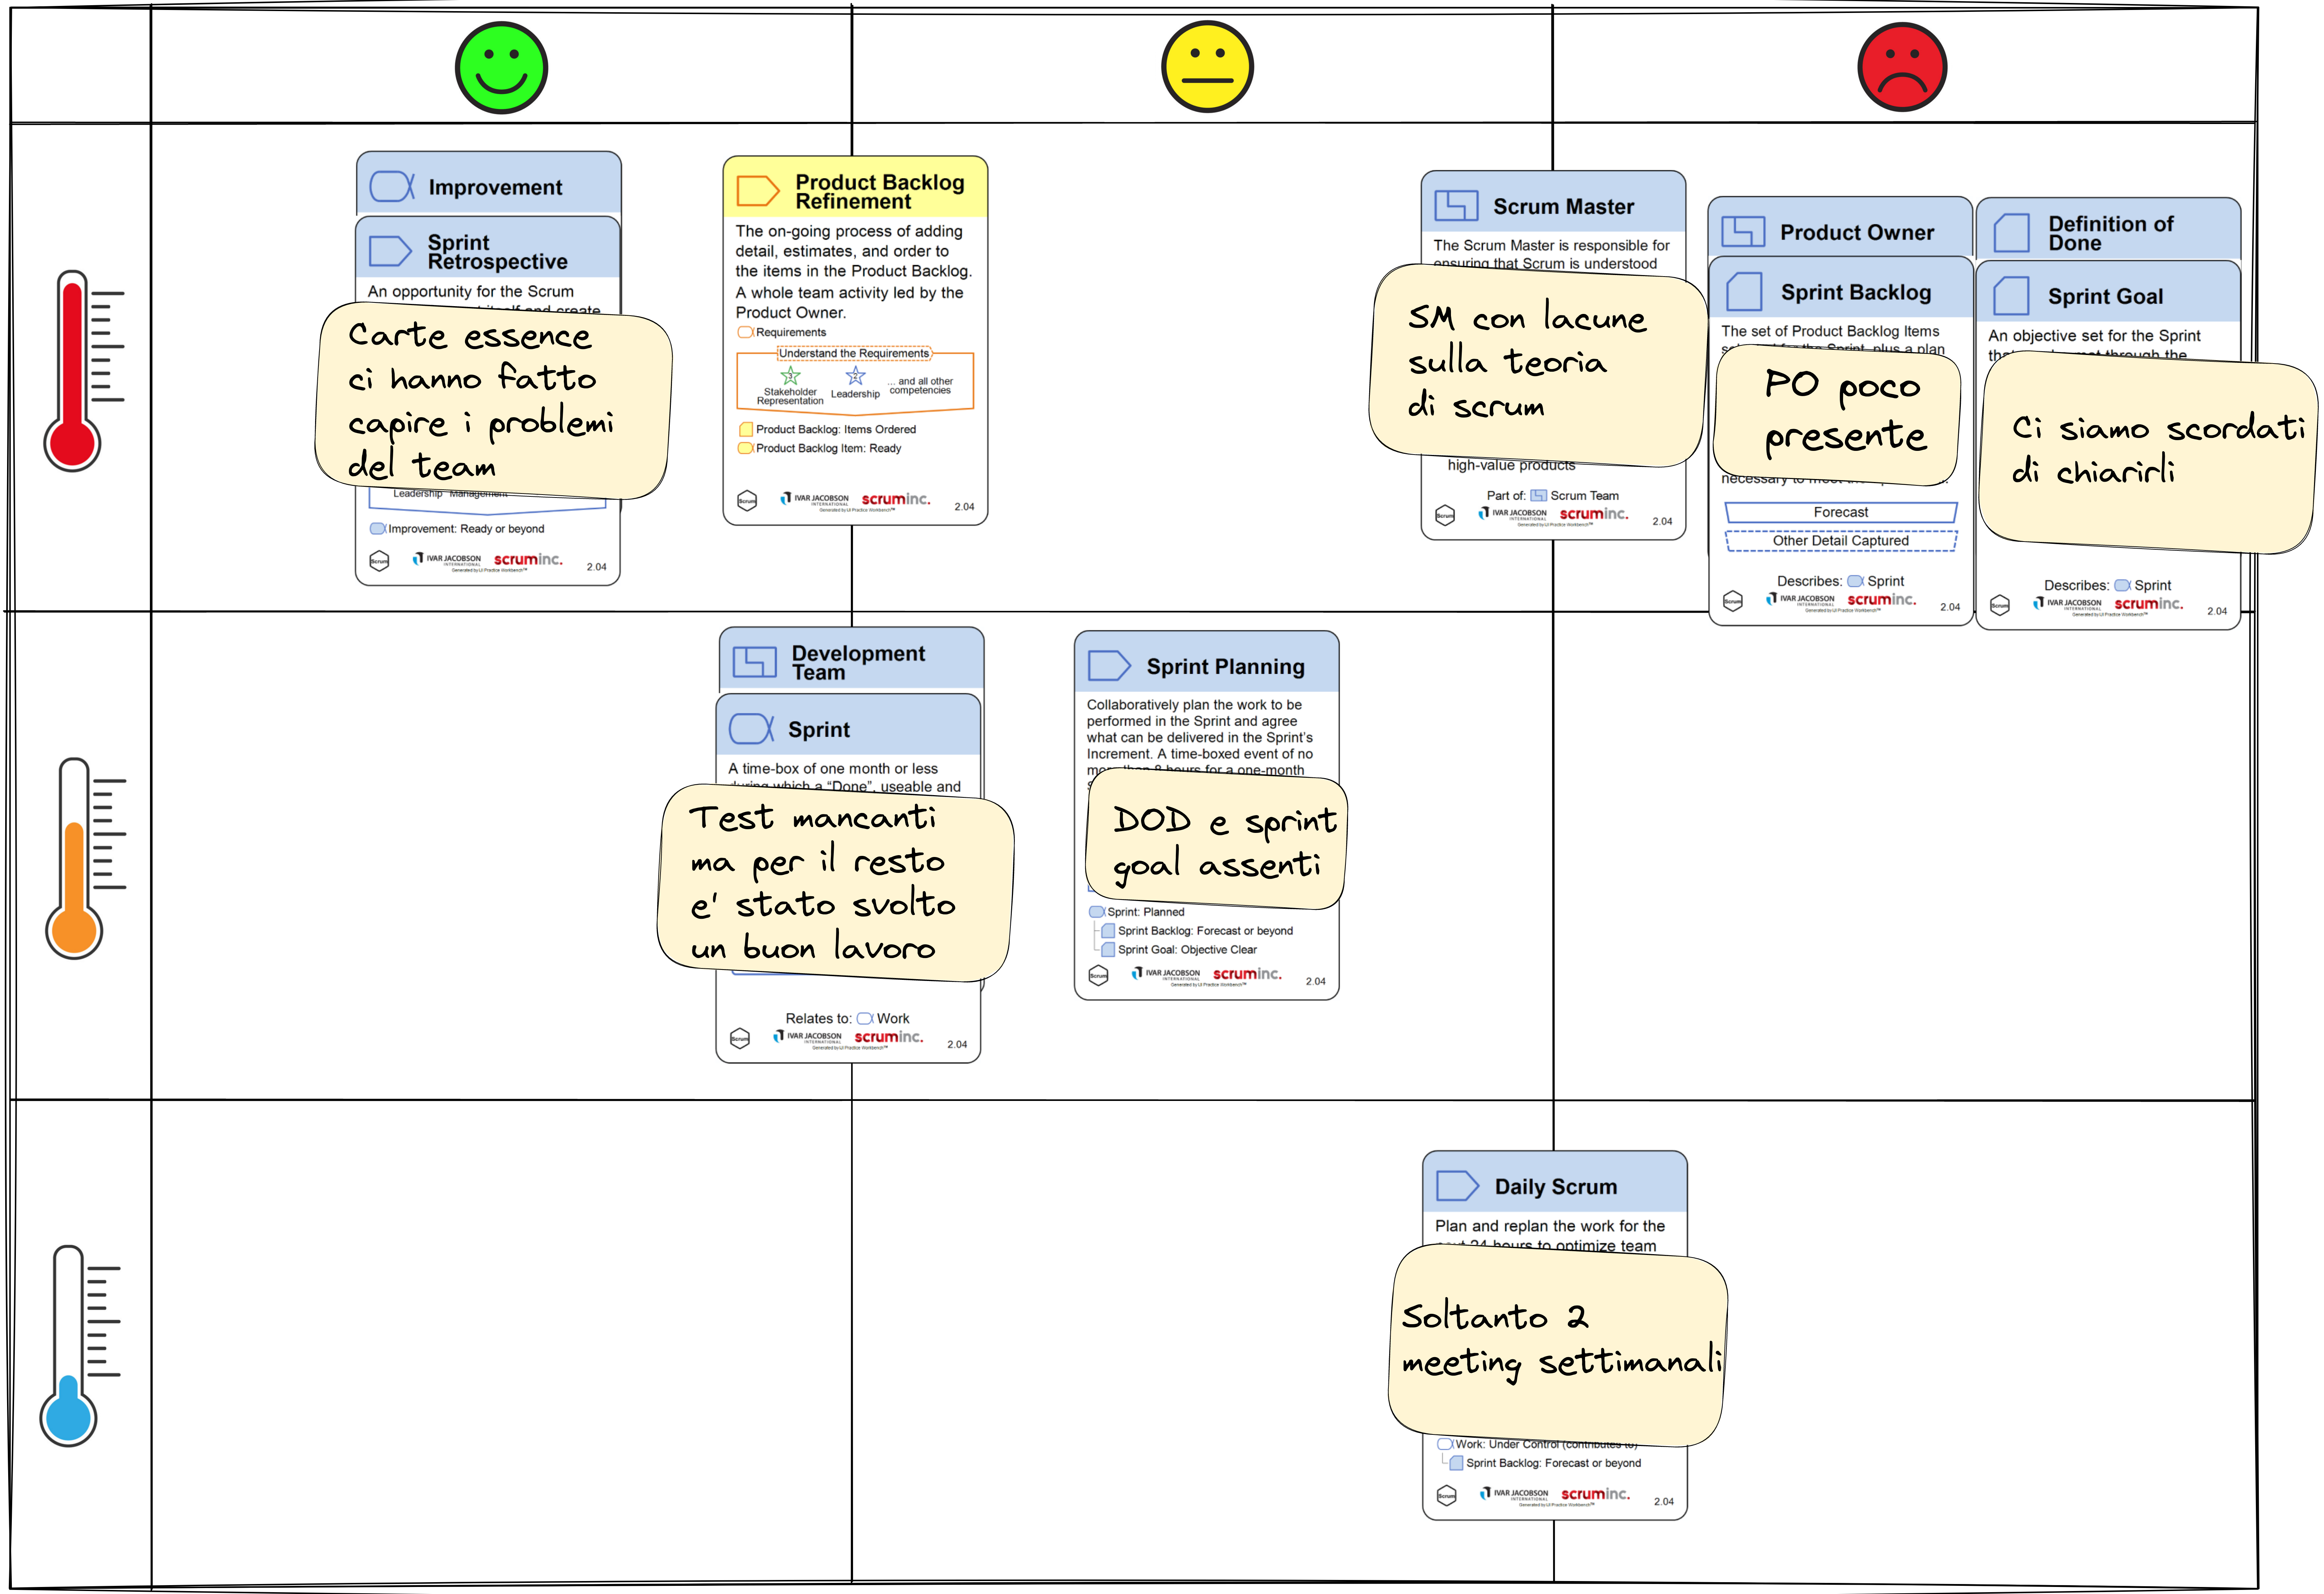
\includegraphics[scale=0.065]{retrospettive/retrospettiva-sprint1.png}
    \caption{Immagine esportata da \href{https://excalidraw.com/}{https://excalidraw.com}}
    \label{fig:retrospettiva1}
\end{figure}

\subsection{Sprint 2}
\subsubsection{Sprint goal}
Abbiamo deciso di fissare il seguente obiettivo da raggiungere durante questo sprint: \\
Portare alla demo un client che permettesse di filtrare ricerche e visualizzare statistiche di sentiment analysis e di distribuzione temporale su tali ricerche. \\
\`E stato un obiettivo abbastanza impegnativo che per fortuna siamo riusciti a raggiungere, con qualche piccola mancanza.
\subsubsection{Sprint backlog}
\begin{itemize}
    \item Come genitore apprensivo vorrei un modo per cercare i tweet di mio figlio per monitorarlo

    \textbf{Stima}: 15 punti
    \item Come analista vorrei avere un grafico che mi permette di vedere il numero di tweet raccolti nel tempo, così da sapere gli andamenti di popolarità dei topic

    \textbf{Stima}: 13 punti
    \item Come genitore apprensivo vorrei un modo per cercare i tweet di mio figlio e visualizzarli sulla mappa
    
    \textbf{Stima}: 13 punti
    \item Come analista di dati vorrei un grafico a torta sul sentiment dei tweet, per farmi un'idea di cosa ne pensino gli utenti
    
    \textbf{Stima}: 28 punti
     \item Come storico, voglio poter scegliere un intervallo di date, per selezionare i tweet del solo periodo che sto studiando
     
    \textbf{Stima}: 14 punti
    \item Come binge tweeter, voglio poter visualizzare piu' di 10 tweet alla volta
    
    \textbf{Stima}: 15 punti
\end{itemize}
\subsubsection{Definition of Done}
Durante questo sprint abbiamo considerato una US \textit{closed} quando venivano rispettati i seguenti punti: 
\begin{itemize}
    \item Il codice che la implementa è stato sufficientemente
commentato.
    \item Il codice rispecchia ció che è scritto nella us.
    \item Il codice è stato visionato da almeno un altro sviluppatore (attraverso le \href{https://docs.gitlab.com/ee/user/project/merge_requests/}{merge requests}).
\end{itemize}
\subsubsection{Burndown dello sprint}
\begin{figure}[H]
    \centering
    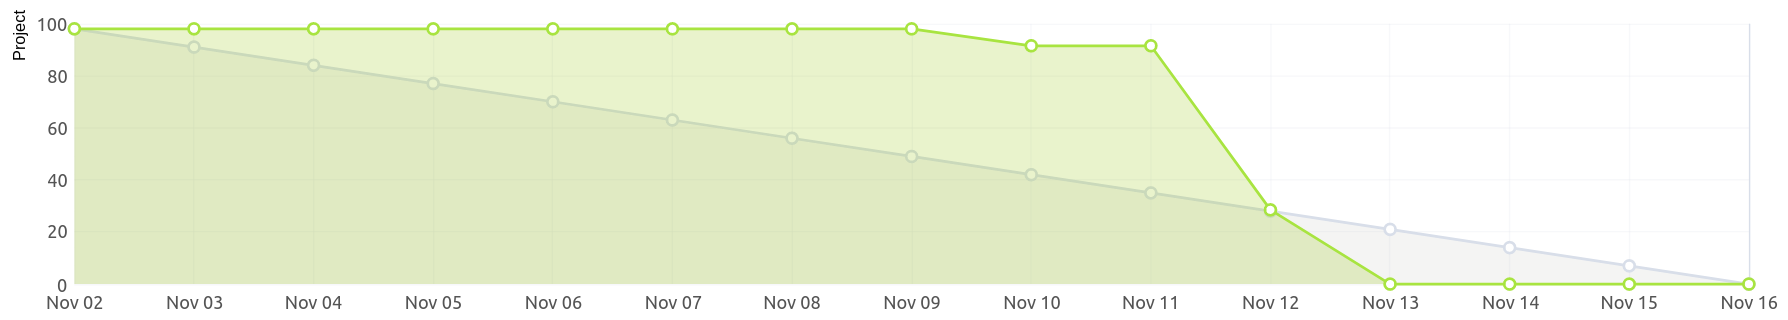
\includegraphics[scale=0.22]{burdowns/sprint2.png}
    \caption{Screenshot da Taiga}
    \label{fig:burndown2}
\end{figure}
Analizzando il burndown, si riescono a notare:
\begin{itemize}
    \item Poca praticit\'a con l'utilizzo di Taiga.
    \item Avendo finito prima del previsto le US di Taiga, abbiamo deciso di non prenderne altre dal product backlog perch\`e sapevamo che non saremmo riusciti a completarle.
    
    Piuttosto ci siamo concentrati sul consolidare le nostre conoscenze di CAS e del testing per JS (\href{https://docs.gitlab.com/ee/ci/pipelines/}{CI/CD Pipelines}, \href{https://docs.sonarqube.org/latest/}{Sonarqube}, \href{https://testing-library.com/docs/react-testing-library/intro/}{React testing library} e \href{https://mswjs.io/docs/api/response}{Mock service worker}) in vista del prossimo sprint.
\end{itemize}
\subsubsection{Test}
A seguire riportiamo uno tra i vari test che abbiamo incluso: \\
\textit{given a query should respond with up to max\_results elements}:

Questo test assicura che quando \`e stato settato il parametro di query \textit{max\_results} vengono restituiti, dalla nostra API, al pi\'u \textit{max\_results} tweet.

\subsubsection{Scelte progettuali}
Durante questo sprint abbiamo deciso di utilizzare:
\begin{itemize}
    \item \href{https://leafletjs.com/}{Leaflet} per la visualizzazione della mappa, inizialmente il nostro team di sviluppatori aveva scelto Google Maps, ma per mantenere coerenza con le altre tecnologie \textit{open source} abbiamo fatto un \textit{refactor} per passare a \textit{Leaflet}.
    \item \href{https://www.npmjs.com/package/multilang-sentiment}{Multilang-sentiment} come libreria per la sentiment analysis.
\end{itemize}
\subsubsection{Sprint Review}
Grazie alla sprint review siamo riusciti a capire alcune lacune del nostro prodotto, tra cui:
\begin{itemize}
    \item ci \`e stato fatto notare il fatto che la nostra visualizzazione fosse “limitata”, il professore voleva una visualizzazione di un grafico a barre dove nell'asse x ci fossero solo i giorni, al pi\'u avrebbe voluto un grafico a barre per minuti.
    \item ci sono stati richiesti i sentimenti dei singoli tweet (per avere una visione piu' chiara delle statistiche, e anche perch\`e cos\'i facendo si riuscirebbe a diminuire l'impressione di \href{https://en.wikipedia.org/wiki/Black_box}{black box})
    \item la nostra ricerca di tweet era limitata a soli 99 tweet, quando le API di twitter ci permettono di chiedere 100 tweet alla volta, per cui ci \`e stato chiesto di aggiungere la possibilit\'a di scegliere 100 tweet.
\end{itemize}
Abbiamo preso atto delle note del professore e le abbiamo implementate nello sprint a seguire.
\subsubsection{Retrospettiva}
Questo sprint \`e andato molto bene rispetto a quello precedente, siamo riusciti a superare le criticita' che erano sorte a fine della restrospettiva dello sprint 1.

Le cose su cui avremmo potuto fare di meglio sono:
\begin{itemize}
\item Lo sprint planning: e' andato abbastanza bene se non fosse per il fatto che abbiamo dovuto tenere un secondo incontro per lo sprint planning poich\`e non eravamo riusciti, per motivi di tempo, a creare i task necessari per le US.
\item La DOD: Abbiamo iniziato a fare test (del backend) ma non li abbiamo inclusi nella DOD perche' non sapevamo quanto sarebbe stato faticoso interfacciarsi con le librerie/framework di testing.
\end{itemize}

Il nostro PO \`e stato un po' assente a causa lavoro ma in fin dei conti non ne ha risentito lo sprint backlog.

Il nostro SM \`e stato molto presente e ha comunicato molto con il team.
\begin{figure}[H]
    \centering
    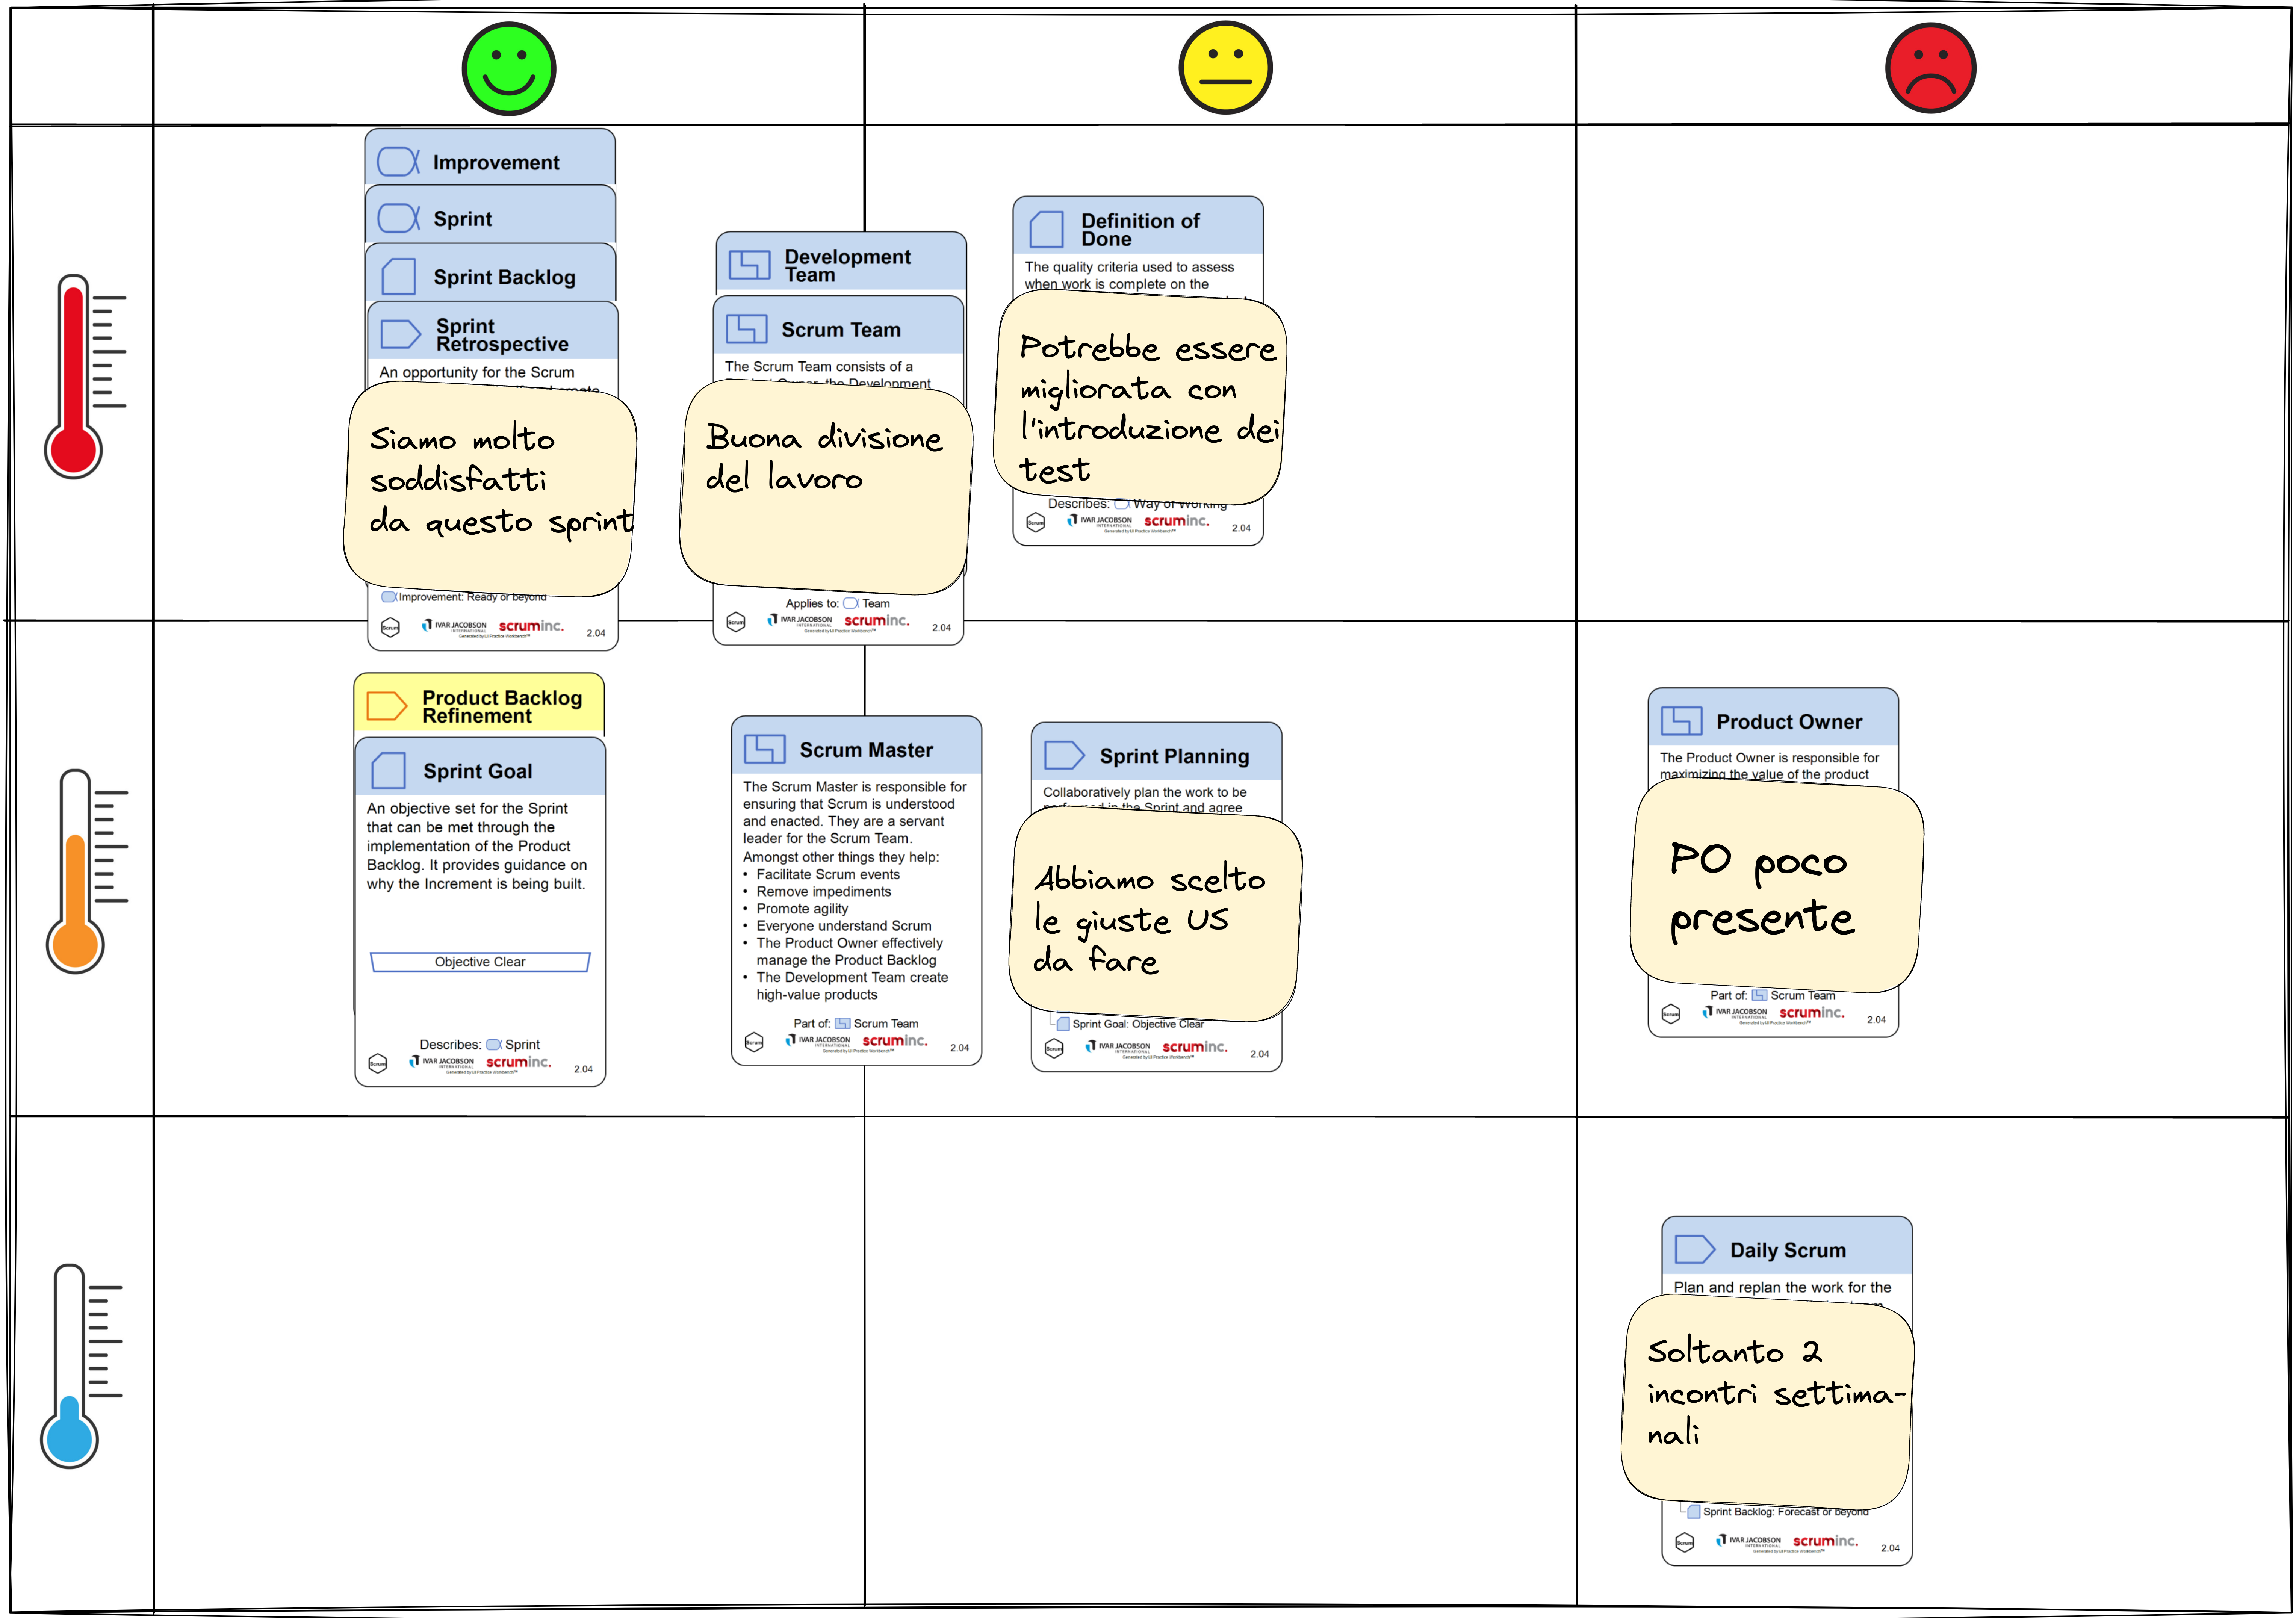
\includegraphics[scale=0.065]{retrospettive/retrospettiva-sprint2.png}
    \caption{Immagine esportata da \href{https://excalidraw.com/}{https://excalidraw.com}}
    \label{fig:retrospettiva2}
\end{figure}
\subsection{Sprint 3}
\subsubsection{Sprint goal}
Lo sprint goal di questo sprint \`e stato il seguente: \\
Avere un client che permettesse di visualizzare statistiche utili, interessanti sulle ricerche effettuate. Inoltre il client deve supportare la visualizzazione dei campioni dell'eredit\'a. \\
A questo punto, per fortuna, eravamo messi abbastanza bene dal punto di vista delle funzionalit\'a implementate, questo ci ha permesso di fissare uno sprint goal "onesto".
\subsubsection{Sprint backlog}
\begin{itemize}
    \item Come membro dell'accademia della crusca vorrei vedere le parole dei tweet selezionati su una term cloud, così da poter vedere le parole più utilizzate

    \textbf{Stima}: 15 punti
    \item Come spettatore de \#leredita (RAI1) voglio raccogliere i tweet di chi prova a indovinare la ghigliottina, per visualizzare (in ordine temporale, o su una mappa) tutti coloro che indovinano
    
    \textbf{Stima}: 32 punti
\end{itemize}
A seguire sono riportate le US che non abbiamo completato
\begin{itemize}
    \item Come giocatore di scacchi voglio sfidare gruppi di persone in rete, per giocare partite le cui mosse verranno scelte a maggioranza

    \textbf{Stima}: 18 punti
    \item Come giocatore di scacchi, voglio raccogliere i tweet che rispondono alla mia mossa, per scegliere e visualizzare la mossa scelta dalla maggioranza

    \textbf{Stima}: 23 punti
\end{itemize}
A seguire sono riportati gli issue che abbiamo risolto, sorti durante la sprint review dello sprint 2.
\begin{itemize}
    \item La card dei singoli tweet va estesa per includere la sentiment analysis del tweet
    \item Gli endpoint che raccolgono i tweet devono fare in modo di poter ritornare fino a 100 tweets
    \item Il diagramma a barre va esteso con la possibilità di avere i minuti come unità di tempo
    \item Il diagramma a barre va esteso con la possibilità di avere i giorni come unità di tempo
\end{itemize}
\subsubsection{Definition of Done}
La DOD \`e rimasta uguale a quella dello sprint scorso, abbiamo provato ad aggiungere anche il seguente punto:
\begin{itemize}
    \item Il codice che implementa la US \`e coperto da test
\end{itemize}
Tuttavia per motivi di tempo (il setup per eseguire i test nel frontend non \`e banale), non siamo riusciti a testare molti componenti del frontend, ci siamo limitati a testarne un paio.
\subsubsection{Burndown dello sprint}
\begin{figure}[H]
    \centering
    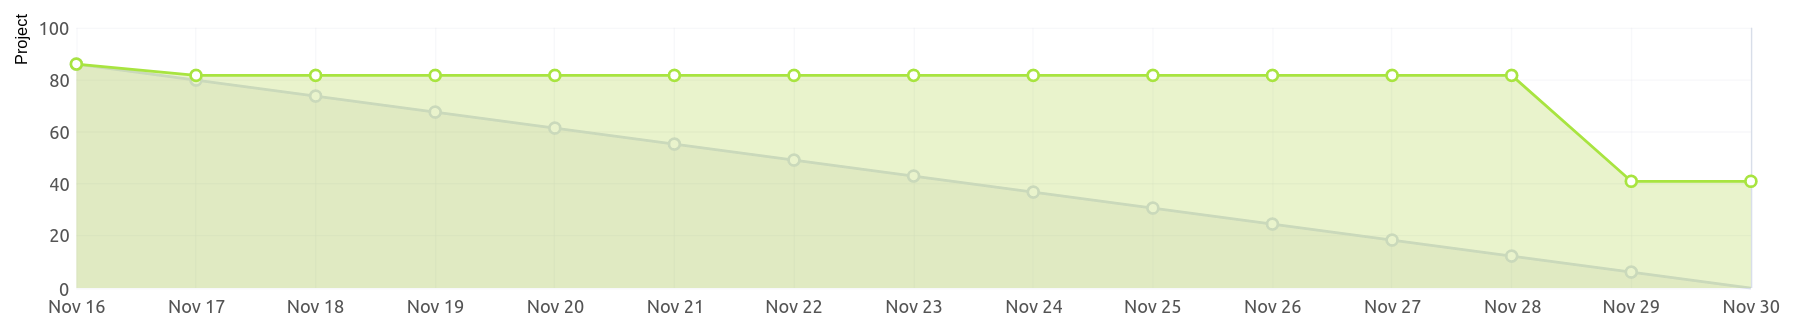
\includegraphics[scale=0.22]{burdowns/sprint3.png}
    \caption{Screenshot da Taiga}
    \label{fig:burndown3}
\end{figure}
Analizzando il burndown, si riescono a notare i seguenti punti:
\begin{itemize}
    \item Sovvracarico di lavoro.
    \item Non siamo riusciti a completare tutte le US e questo ci ha fatto accumulare debito tecnico che si \`e concretizzato nell'implementazione di pochi test per la nostra codebase.
\end{itemize}
\subsubsection{Test}
A seguire riportiamo due esempi di test del backend e del frontend, rispettivamente : \\
\textit{should return an array of wordcloud info if input tweets are provided}:

Questo test assicura che venga creato un array contenente le informazioni di wordcloud che ci interessano. \\
\textit{SearchForm component should show filters when they're enabled}:

Questo test assicura che il componente SearchForm renda visibili i filtri di ricerca se vengono abilitati
\subsubsection{Scelte progettuali}
Durante questo sprint abbiamo deciso di utilizzare:
\begin{itemize}
    \item Abbiamo deciso di reperire le informazioni sulla ghigliottina dall'account twitter che posta tutti i giorni le risposte giuste e i relativi campioni: \href{https://twitter.com/quizzettone}{https://twitter.com/quizzettone}
    \item Al backend \`e stato eseguito un refactor per fare in modo che venisse utilizzato \href{https://github.com/PLhery/node-twitter-api-v2}{node-twitter-api-v2} come client per interfacciarsi con le API di twitter, questo ci ha aiutato a gestire al meglio gli stream.
    \item \href{https://github.com/Clariity/react-chessboard}{react-chessboard} come componente per la scacchiera lato frontend e \href{https://github.com/jhlywa/chess.js}{chess.js} come libreria per gestire la logica degli scacchi.
    \item \href{https://www.npmjs.com/package/chess-image-generator}{chess-image-generator} come libreria per la generazione delle immagini delle scacchiere dati FEN, PGN o array (a noi \`e venuto comodo utilizzare \textit{.loadFEN(fen)} ).
    \item Poich\'e non avevamo a disposizione nessuna macchina su cui fare il deployment della nostra applicazione, abbiamo deciso richiedere uno spazio web al DISI (\href{https://disi.unibo.it/it/dipartimento/servizi-tecnici-e-amministrativi/servizi-informatici/gruppi-spazi-web-e-database}{da qui}). \\
    Ci \`e stato assegnato l'indirizzo \href{http://site212236.tw.cs.unibo.it}{http://site212236.tw.cs.unibo.it}
\end{itemize}
\subsubsection{Pipeline}
In questo sprint, Juan si \`e occupato di implementare la pipeline per la continuous integration, testing e deployment. (a tal proposito \`e stato molto utile consultare la documentazione ufficiale di gitlab: \href{https://docs.gitlab.com/ee/ci/pipelines/}{pipelines} )
\begin{figure}[H]
    \centering
    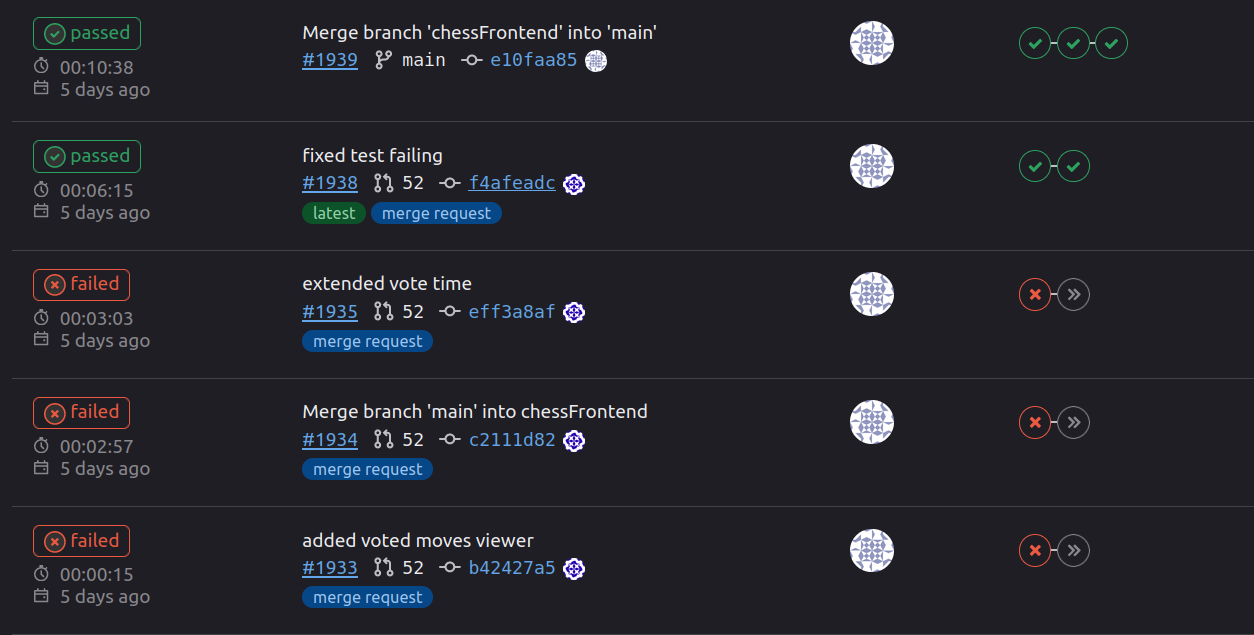
\includegraphics[scale=0.25]{misc/example_pipeline.png}
    \caption{Screenshot da gitlab}
    \label{fig:pipeline}
\end{figure}
\subsubsection{Sprint Review}
Il 5/12/2022 abbiamo tenuto il secondo incontro con il professore per lo stato di avanzamento del prodotto durante lo sprint 3.

Durante la discussione il professore \`e sembrato entusiasta e soddisfatto per il nostro stato di avanzamento.

La discussione col professore \`e andata molto bene e la demo \`e piaciuta.
\subsubsection{Retrospettiva}
Questo sprint \`e andato bene anche se non siamo riusciti a completare tutte le US dello sprint backlog perch\'e abbiamo sottovalutato la complessit\'a delle US degli scacchi.

Le cose da migliorare sono state:
\begin{itemize}
    \item La stima dell'effort necessario per completare le US
    \item La situazione dei test del frontend (anche se e' stato veramente complesso settare l'ambiente di test e questo ci ha rallentati parecchio) e del backend
\end{itemize}
\begin{figure}[H]
    \centering
    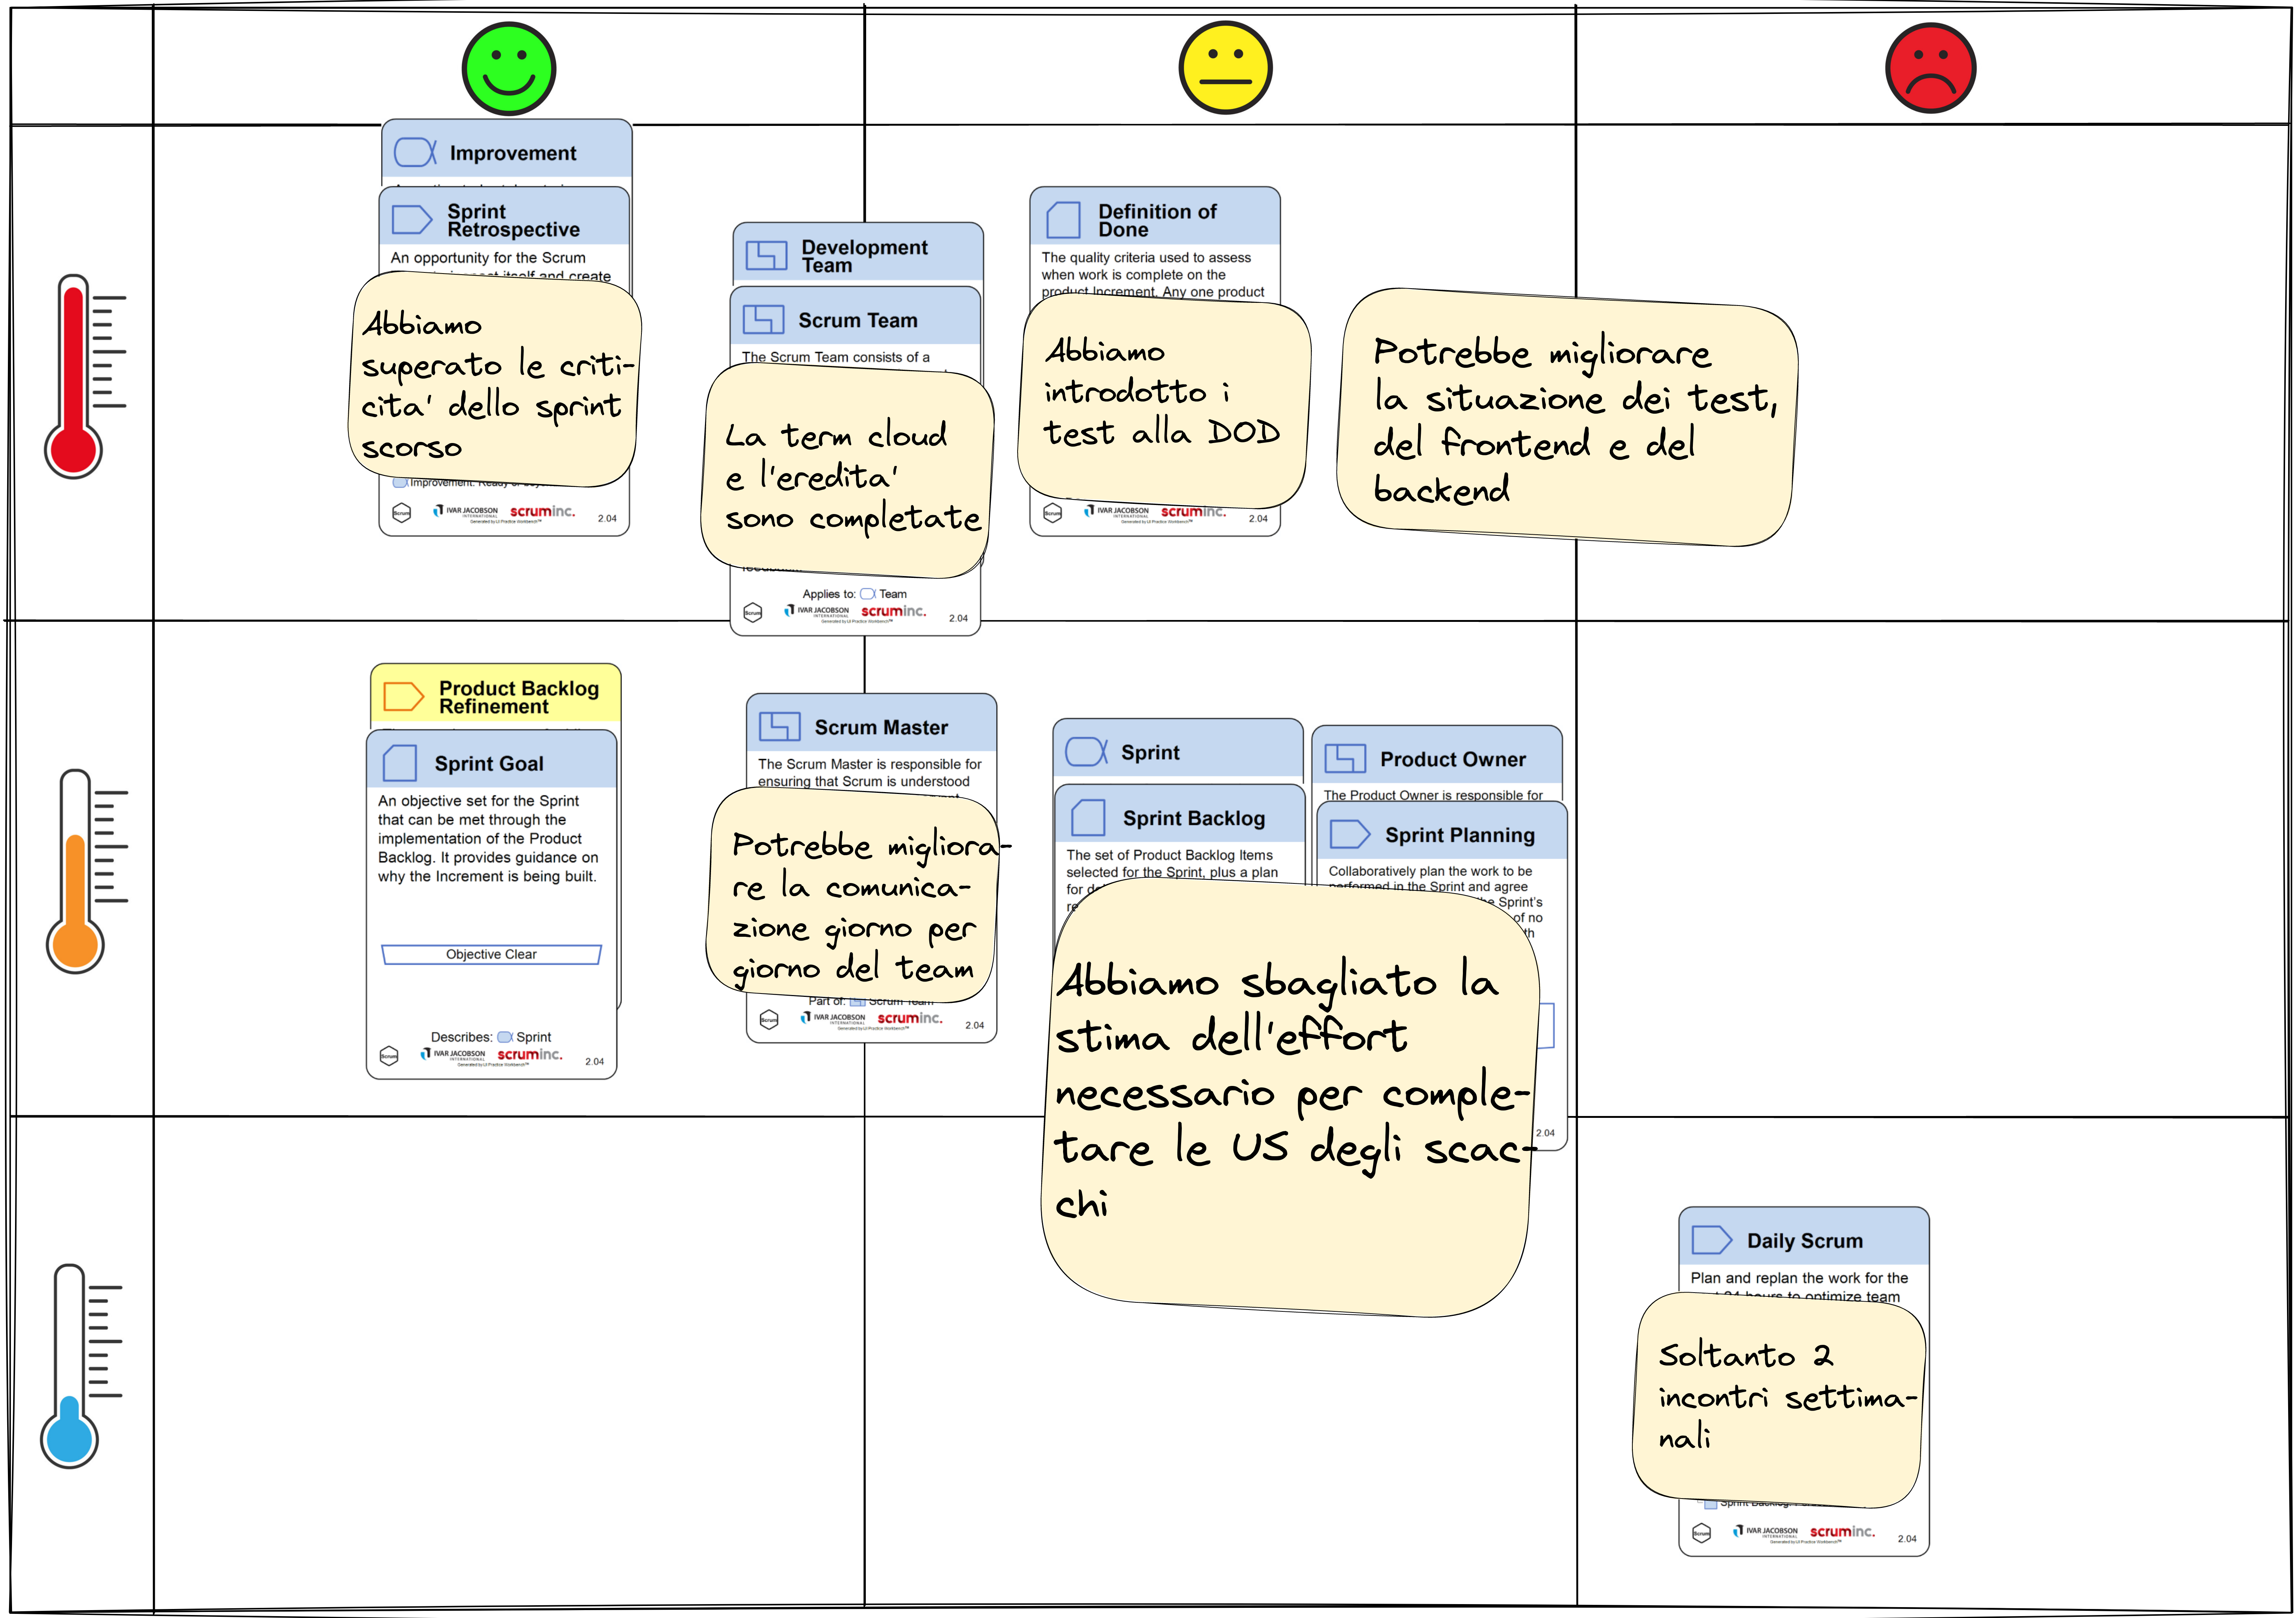
\includegraphics[scale=0.065]{retrospettive/retrospettiva-sprint3.png}
    \caption{Immagine esportata da \href{https://excalidraw.com/}{https://excalidraw.com}}
    \label{fig:retrospettiva3}
\end{figure}
\subsection{Sprint 4}
\subsubsection{Sprint goal}
Le nostre intenzioni sono state fin dall'inizio quelle di consegnare il progetto a Dicembre, perci\'o questo sprint ha avuto come obiettivo: \\
Avere un client che permetta di giocare a scacchi tramite l'utilizzo di tweet e che permetta di ottenere informazioni interessanti sul fantacitorio.
\subsubsection{Sprint backlog}
\begin{itemize}
    \item Come giocatore di scacchi voglio sfidare gruppi di persone in rete, per giocare partite le cui mosse verranno scelte a maggioranza

    \textbf{Stima}: 18 punti
    \item Come giocatore di scacchi, voglio raccogliere i tweet che rispondono alla mia mossa, per scegliere e visualizzare la mossa scelta dalla maggioranza

    \textbf{Stima}: 23 punti
    \item Come spettatore del fantacitorio voglio poter visualizzare la classifica emendabile settimanale / di sempre dei politici.

    \textbf{Stima}: 26 punti
    \item Come spettatore del fantacitorio voglio poter vedere le squadre dei miei amici

    \textbf{Stima}: 19 punti
    \item Come spettatore del fantacitorio voglio poter sfogliare le immagini delle squadre registrate

    \textbf{Stima}: 24 punti
\end{itemize}
\subsubsection{Definition of Done}
La DOD \`e rimasta uguale a quella dello sprint scorso.
Siamo riusciti a testare gran parte del backend, purtroppo non possiamo dire lo stesso del frontend: \\ per testare tutti i componenti del frontend, ci sarebbe voluto un altro sprint.
\subsubsection{Burndown dello sprint}
\begin{figure}[H]
    \centering
    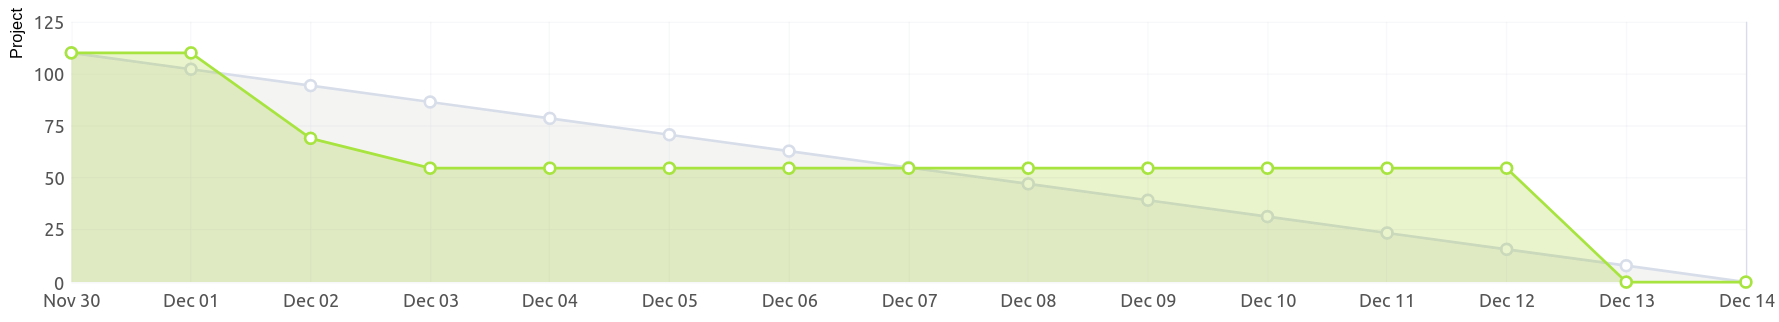
\includegraphics[scale=0.22]{burdowns/sprint4.png}
    \caption{Screenshot da Taiga}
    \label{fig:burndown4}
\end{figure}

\subsubsection{Test}
A seguire riportiamo due esempi di test del backend e del frontend, rispettivamente : \\
\textit{should return an array of objects with the politicians and their summed points with full names}:

Questo test assicura che venga creato un array contenente le informazioni per la classifica del fantacitorio che ci interessano. \\
\textit{form utils' isValidDateRange function should work as expected w/valid ranges}:

Questo test assicura che il la funzione isValidDateRange (utilizzata quando viene effettuata una ricerca, per controllare che l'intervallo delle date sia valido) validi i range di date correttamente.
\subsubsection{Scelte progettuali}
\begin{itemize}
    \item Abbiamo deciso di reperire le informazioni sul fantacitorio dall'account twitter del fantacitorio: \href{https://twitter.com/Fanta_citorio}{https://twitter.com/Fanta\_citorio}
    \item Per fare in modo di supportare la richiesta del prof della classifica non solo dell'ultima settimana, abbiamo utilizzato \\ \href{https://developer.twitter.com/en/docs/twitter-api/users/lookup/api-reference/get-users-id}{https://developer.twitter.com/en/docs/twitter-api/users/lookup/api-reference/get-users-id}. \\
    Questo endpoint ci permette di ricavare i tweet di un utente senza limitazioni sull'arco temporale (i.e. siamo riusciti a soddisfare la richiesta del prof senza utilizzare basi di dati di appoggio). \\
\end{itemize}
\subsubsection{Retrospettiva}
Questo sprint \`e andato bene, siamo riusciti a completare lo sprint goal che ci eravamo prefissati (i.e. consegnare il progetto prima di natale), ma ci sono state comunque delle cose che avremmo potuto fare meglio:
\begin{itemize}
\item La comunicazione del team: abbastanza cruciale per questo ultimo sprint, \`e stata scarsa da parte di alcuni componenti del team.
\item La DOD: Abbiamo testato al dettaglio il backend, purtroppo non siamo riusciti a fare lo stesso per il frontend poich\'e ci sarebbe voluto un altro sprint per aumentare la coverage dei nostri componenti.
\end{itemize}
\begin{figure}[H]
    \centering
    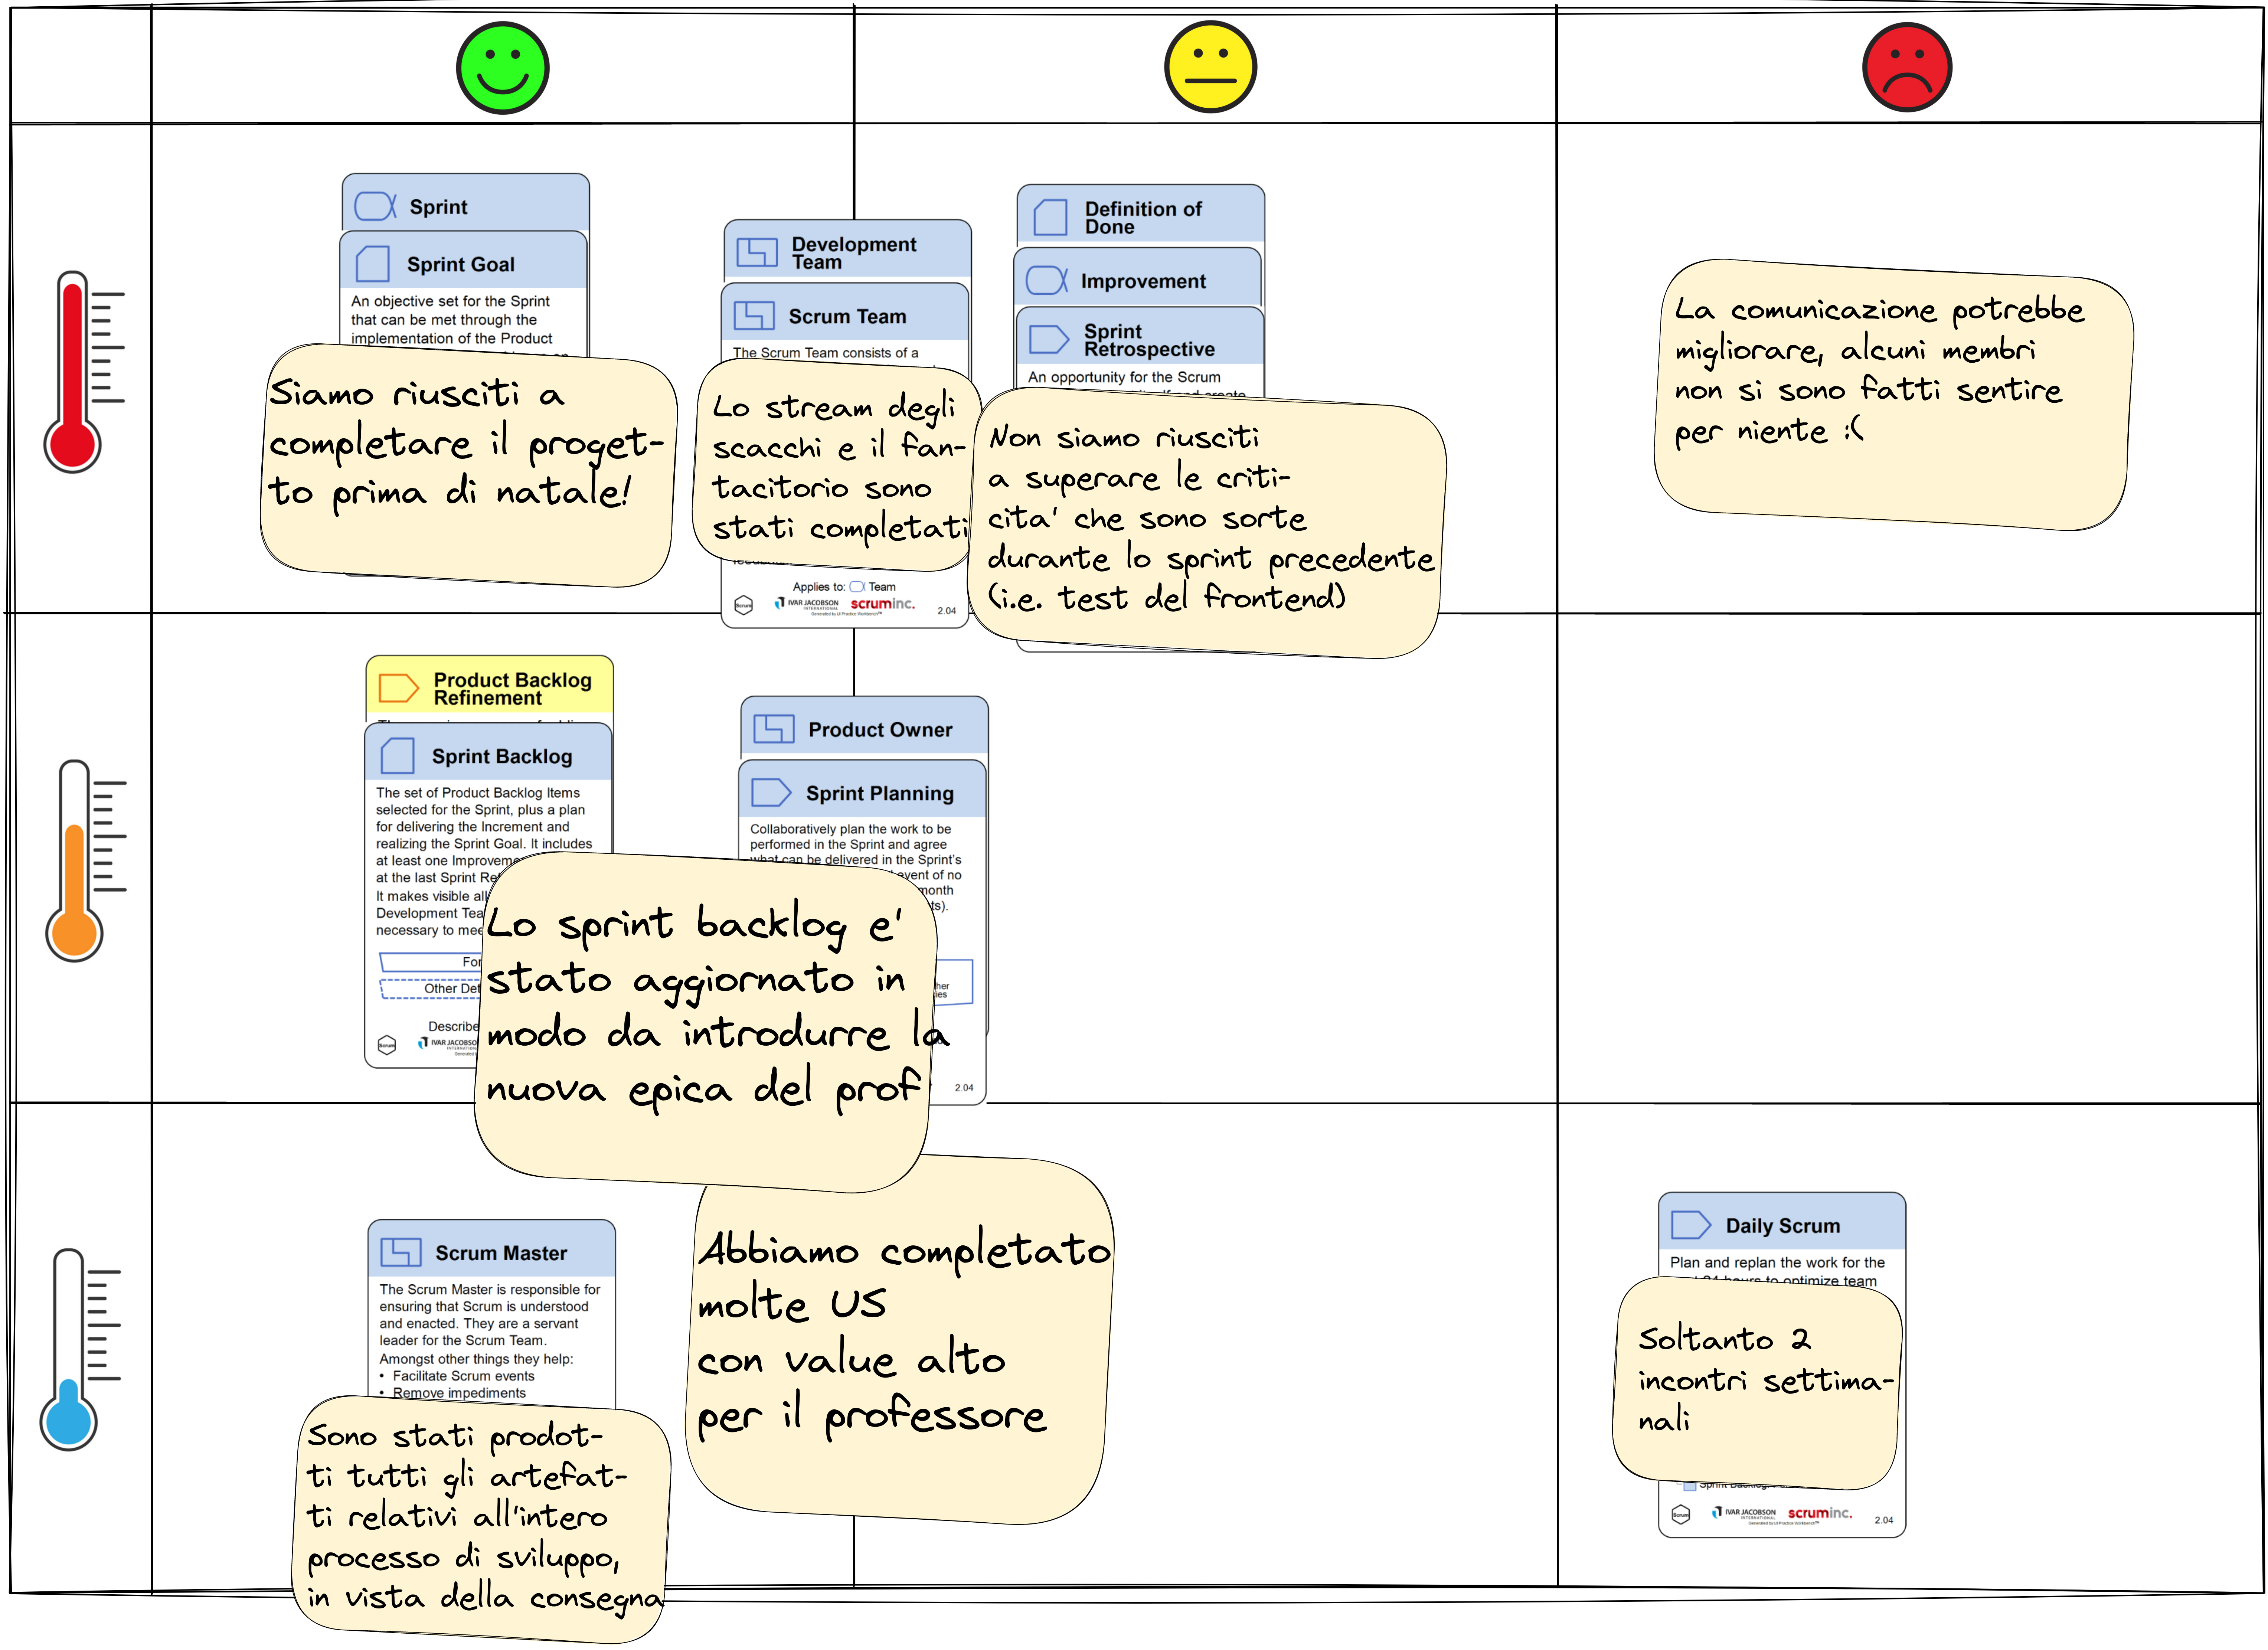
\includegraphics[scale=0.065]{retrospettive/retrospettiva-sprint4.png}
    \caption{Immagine esportata da \href{https://excalidraw.com/}{https://excalidraw.com}}
    \label{fig:retrospettiva4}
\end{figure}
\subsection{Alcuni dati sul processo}
\subsubsection{Sonarqube}
\begin{figure}[H]
    \centering
    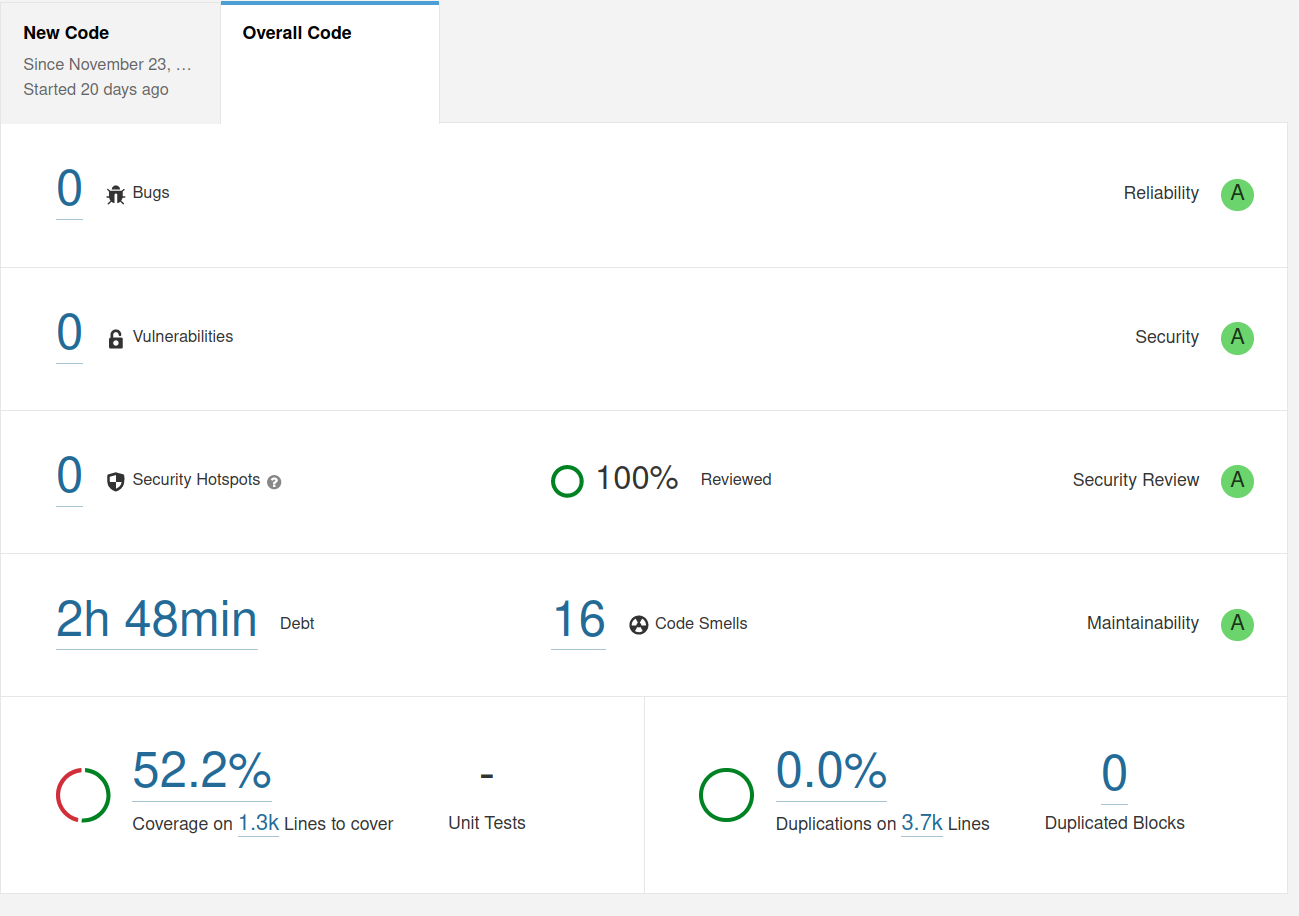
\includegraphics[scale=0.30]{misc/qube_analysis.png}
    \label{fig:qubeanalysis}
\end{figure}
\begin{figure}[H]
    \centering
    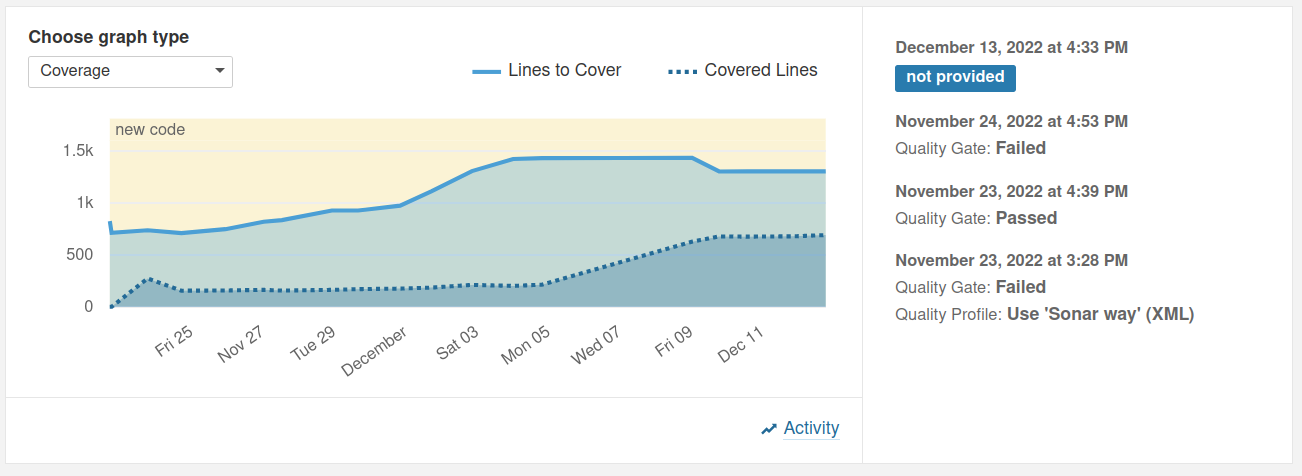
\includegraphics[scale=0.30]{misc/coverage_graph.png}
    \caption{Screenshot della dashboard dell'istanza di sonarqube su \href{https://qube.hjkl.gq}{qube.hjkl.gq}}
    \label{fig:qubeanalysis}
\end{figure}
\subsubsection{Gitinspector}
\begin{figure}[H]
    \centering
    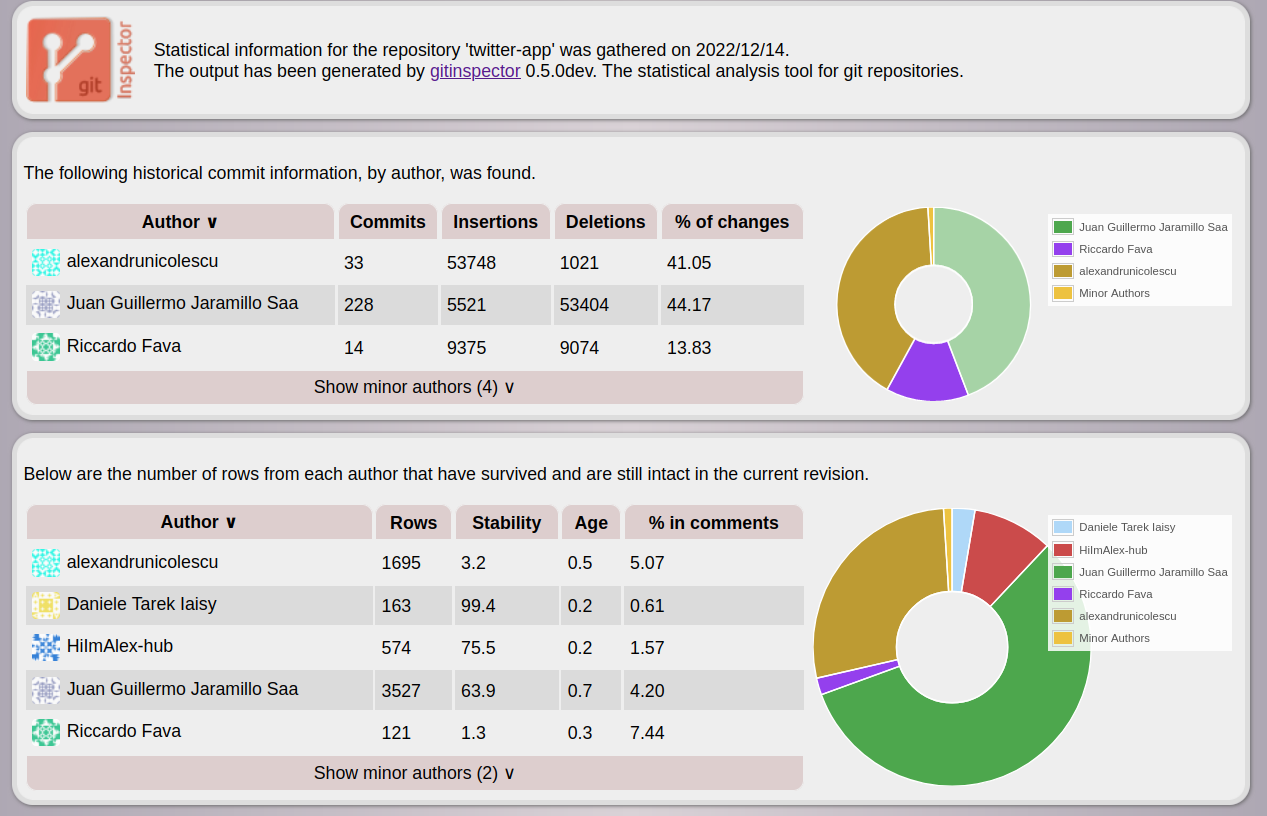
\includegraphics[scale=0.30]{misc/inspector_finale.png}
    \caption{Screenshot dell'output di gitinspector}
    \label{fig:qubeanalysis}
\end{figure}
\subsubsection{Burndown finale}
\begin{figure}[H]
    \centering
    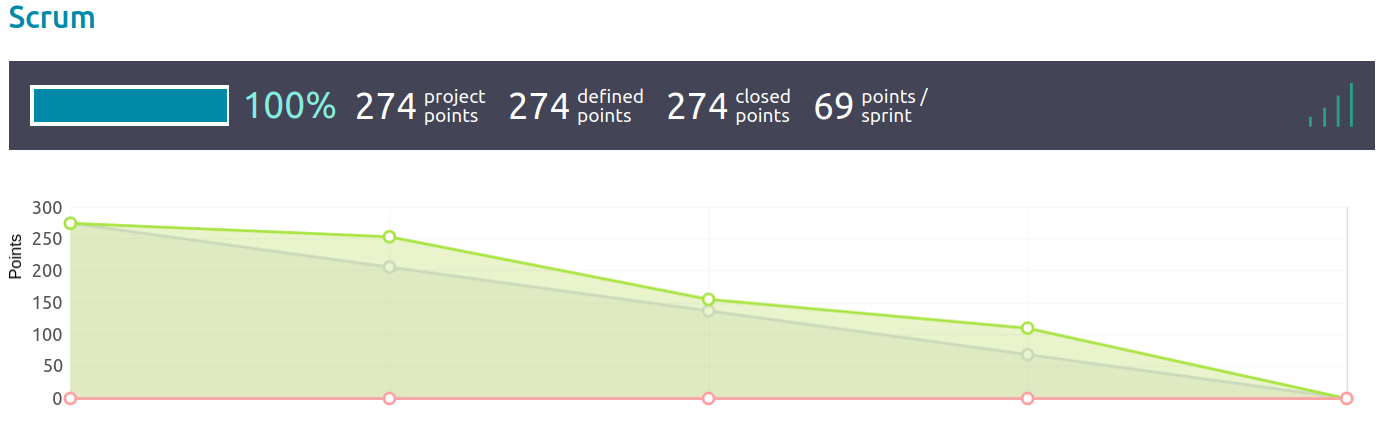
\includegraphics[scale=0.22]{burdowns/burndown_finale.png}
    \caption{Screenshot da Taiga}
    \label{fig:burndown_finale}
\end{figure}
\pagebreak
\section{Artefatti}
\begin{itemize}
    \item \textbf{Link del sito di produzione}: \href{http://site212236.tw.cs.unibo.it/}{http://site212236.tw.cs.unibo.it/}
    \item \textbf{Link all'account twitter dell'app}: \href{https://twitter.com/ingsw2022team3}{https://twitter.com/ingsw2022team3}
    \item \textbf{Video della demo}: \href{https://peertube.devol.it/w/7AnJMxZ3cREsUiyzgREu5X}{https://peertube.devol.it/w/7AnJMxZ3cREsUiyzgREu5X}
    \item \textbf{Taiga del progetto}: \href{https://taiga.hjkl.gq/project/ingsw2022-team3/timeline}{https://taiga.hjkl.gq/project/ingsw2022-team3/timeline}
    \item \textbf{Wiki del progetto}: \href{https://taiga.hjkl.gq/project/ingsw2022-team3/wiki/home}{https://taiga.hjkl.gq/project/ingsw2022-team3/wiki/home}
    \item \textbf{Retrospettive}: \href{https://taiga.hjkl.gq/project/ingsw2022-team3/wiki/retrospettive}{https://taiga.hjkl.gq/project/ingsw2022-team3/wiki/retrospettive}
    \item \textbf{Gitlab}: \href{https://git.hjkl.gq/team3/twitter-app}{https://git.hjkl.gq/team3/twitter-app}
    \item \textbf{Continuous Integration - Continuous Testing - Continuous Deployment}: \href{https://git.hjkl.gq/team3/twitter-app/-/blob/main/.gitlab-ci.yml}{https://git.hjkl.gq/team3/twitter-app/-/blob/main/.gitlab-ci.yml}
    \item \textbf{Eseguire in locale}: \href{https://git.hjkl.gq/team3/twitter-app/-/blob/main/README.md}{https://git.hjkl.gq/team3/twitter-app/-/blob/main/README.md}
    \item \textbf{Sonarqube}: \href{https://qube.hjkl.gq/dashboard?id=team3_twitter-app_AYP2_cazVcJsoVycNZv6}{link a sonarqube}

\end{itemize}

\end{document}
